%% Manuscript for Science of Computer Programming (Elsevier), research paper.
%% Build: make (figures, then latexmk). Class: elsarticle v3.5 (bundled here), numbered references.
\documentclass[preprint,12pt,sort&compress,nopreprintline]{elsarticle}

\usepackage{lmodern}
\usepackage[T1]{fontenc}
\usepackage[utf8]{inputenc}
\usepackage{amsmath,amssymb,amsthm}
\usepackage{mathpartir}
\usepackage{booktabs}
\usepackage{tabularx}
\usepackage{multirow}
\usepackage{graphicx}
\usepackage{xcolor}
\usepackage{listings}
\usepackage{microtype}
\usepackage{enumitem}
\usepackage[switch]{lineno}
\usepackage[hidelinks]{hyperref}
\usepackage[capitalise,nameinlink,noabbrev]{cleveref}
\pdfstringdefDisableCommands{\def\corref#1{}\def\fnref#1{}}

\journal{Science of Computer Programming}

%% Cross-reference names in the journal's style: "Fig. 3", "Section 4", "Table 2".
\crefname{figure}{Fig.}{Figs.}
\Crefname{figure}{Fig.}{Figs.}
\crefname{section}{Section}{Sections}
\crefname{appendix}{Appendix}{Appendices}
\crefname{table}{Table}{Tables}
\crefname{lstlisting}{Listing}{Listings}

%% Theorem-like environments, numbered separately.
\theoremstyle{plain}
\newtheorem{theorem}{Theorem}
\newtheorem{lemma}{Lemma}
\newtheorem{proposition}{Proposition}
\newtheorem{corollary}{Corollary}
\theoremstyle{definition}
\newtheorem{definition}{Definition}
\newtheorem{example}{Example}
\crefname{theorem}{Theorem}{Theorems}
\crefname{lemma}{Lemma}{Lemmas}
\crefname{proposition}{Proposition}{Propositions}
\crefname{corollary}{Corollary}{Corollaries}
\crefname{definition}{Definition}{Definitions}
\crefname{example}{Example}{Examples}

%% OrchLang listings.
\definecolor{kw}{HTML}{0B3D91}
\definecolor{str}{HTML}{7A3E00}
\definecolor{cmt}{HTML}{5A5A5A}
\lstdefinelanguage{OrchLang}{
  morekeywords={workflow,budget,leaks,observer,input,secret,model,prompt,tool,let,call,using,
    if,else,retry,emit,output,endorse,declassify,as,because,require,tokens,untrusted,
    max_tokens,max_bytes,tokenizer,overhead,mock,text,boolean},
  morestring=[b]",
  morecomment=[l]{//},
  sensitive=true}
\lstset{
  language=OrchLang,
  basicstyle=\ttfamily\footnotesize,
  keywordstyle=\color{kw}\bfseries,
  stringstyle=\color{str},
  commentstyle=\color{cmt}\itshape,
  columns=fullflexible,
  keepspaces=true,
  showstringspaces=false,
  numbers=left, numberstyle=\scriptsize\color{cmt}, numbersep=6pt, xleftmargin=16pt,
  frame=tb, framerule=0.4pt, aboveskip=6pt, belowskip=4pt,
  escapeinside={(*}{*)}}
\newcommand{\code}[1]{\texttt{#1}}
\DeclareRobustCommand{\file}[1]{\path{#1}}

%% Notation.
\newcommand{\Prov}{\mathcal{P}}
\newcommand{\sig}{\mathit{sig}}
\newcommand{\sigv}[1]{\mathit{sig}_{#1}}
\newcommand{\bytes}{\mathit{bytes}}
\newcommand{\tok}{\mathit{tokens}}
\newcommand{\capm}{\mathit{cap}}
\newcommand{\Call}{\mathsf{Call}}
\newcommand{\Retry}{\mathsf{Retry}}
\newcommand{\Branch}{\mathsf{Branch}}
\newcommand{\ptext}{\mathsf{text}}
\newcommand{\pvar}{\mathsf{var}}
\newcommand{\pres}{\mathsf{res}}
\newcommand{\Pub}{\mathrm{P}}
\newcommand{\Sec}{\mathrm{S}}
\newcommand{\Tru}{\mathrm{T}}
\newcommand{\Unt}{\mathrm{U}}
\newcommand{\conf}{\mathsf{C}}
\newcommand{\integ}{\mathsf{I}}
\newcommand{\eps}{\varepsilon}

\begin{document}

\begin{frontmatter}

\title{Compare the requests, not their sizes: Resource side channels and sound token bounds for LLM workflows}

\author[vit]{Nambi Rajan M\corref{cor}}
\ead{AUTHOR-EMAIL} %% TODO(author): corresponding e-mail address
\cortext[cor]{Corresponding author.}
\affiliation[vit]{organization={Vellore Institute of Technology},
            city={Vellore},
            state={Tamil Nadu},
            country={India}} %% TODO(author): school/department and postcode

\begin{abstract}
A program that orchestrates calls to a large language model (LLM) can leak a
secret without the secret reaching a prompt: if the secret decides which
requests are sent, whoever sees the network traffic or the bill can learn it.
Resource-aware noninterference handles such channels by charging each operation
a cost determined by input sizes. We show that this cannot work for LLM calls. Any analysis that sees prompt text only through a size measure is
either unsound for providers whose answers depend on content, or rejects a
secret-guarded branch whose two arms are identical. The theorem is mechanised in
Coq and explains why two size-based rules of our own failed. We compare
requests by content instead, resolving each secret branch by the outcomes its
secret can realise. If every resolution sends the same requests, the workflow is
noninterfering for every provider, tokenizer and observer of its transcript; if
$k$ request classes remain, it leaks at most $\log_2 k$ bits of min-capacity.
Because tokenization is not subadditive, we compute worst-case token bounds in
bytes and convert them through contracts measured on fourteen tokenizers. Both
analyses are implemented in OrchLang, a small workflow language, and evaluated on
synthetic suites and on thirty workflows ported from
LangGraph, the Anthropic cookbook and AgentDojo under a protocol fixed before
porting. No certified bound was exceeded in 6,000 runs of the ported workflows.
None of them has a secret, so the relational analysis has so far been exercised
only on synthetic workflows.
\end{abstract}


\begin{keyword}
Information flow \sep Resource side channels \sep Relational analysis \sep
Quantitative information flow \sep Tokenization \sep Large language models \sep Coq
\end{keyword}

\end{frontmatter}

\linenumbers

\section{Introduction}\label{sec:intro}

\Cref{fig:triage} shows a customer-support workflow written in OrchLang, the
language this paper is about. It answers a ticket with a small model. When the
customer's account carries a private fraud-risk flag, \code{high\_risk}, it also
asks a larger model to check the reply before the reply is sent. The flag never
reaches a prompt, the workflow's output or the tool that sends the reply. An
information-flow type system with a program-counter label therefore has nothing
to object to: nothing observable at a sink depends on the flag.

The requests do depend on it. For a customer with the flag set, the workflow makes
two requests, one of them to a more expensive model; for everyone else it makes
one. The provider bills per model, so a tenant's invoice shows which customers
were checked. An observer of the encrypted traffic sees request and response
sizes, from which token-length and packet-size attacks have recovered response
text and prompt topics~\cite{weiss2024what,mcdonald2025whisper}, and a
prompt cache shared between users turns the same requests into a timing
channel~\cite{gu2025auditing}. Each of these observers sees a function of the
workflow's requests and responses. If a secret changes the requests, it can change
what they see, even when no secret value crosses any boundary.

\begin{figure}[t]
\lstinputlisting[basicstyle=\ttfamily\footnotesize]{examples/triage.orch}
\vspace{-2pt}
{\scriptsize\ttfamily\raggedright\hangindent=1.5em%% Generated by examples/run.py from `orchc check triage.orch`. Do not edit.
triage.orch:13:3: error [E236] the guard 'high\_risk' depends on a secret and the two arms send different requests, so the trace observer can tell which arm ran; one arm makes 1 top-level request(s), the other 0. then-arm sends [openai/gpt-4o("Check this reply for mistakes: " + reply)] and else-arm sends [nothing]
\par}
\caption{The running example and the compiler's verdict. The secret \code{high\_risk} never
reaches a prompt, an output or a tool, yet it decides whether the second request is sent.
With the header \code{workflow Triage budget 1000000 leaks 1} the same program is accepted
with a warning that it reveals at most one bit (\cref{sec:quantitative}); without the
\code{endorse} on lines 16--17 it is rejected earlier, because text derived from the untrusted
ticket would drive the tool (\cref{sec:language}).}
\label{fig:triage}
\end{figure}

\subsection{Why the classical treatment does not transfer}\label{sec:intro-classical}

This is a resource side channel, and its classical treatment is mature. Ngo,
Dehesa-Azuara, Fredrikson and Hoffmann define resource-aware noninterference and
constant resource, and certify both by combining information-flow typing with
automatic amortised resource analysis (AARA)~\cite{ngo2017verifying}. Çiçek,
Barthe, Gaboardi, Garg and Hoffmann's RelCost bounds the difference in cost
between two executions with relational refinement types~\cite{cicek2017relational}.
Ngo et al.\ quantify over environments that agree on the sizes of secret data, and
RelCost bounds cost differences in terms of sizes and of how much two inputs
differ. Both charge each operation a cost that the program's data determine.

The cost of an LLM call is not determined by sizes. Two requests of exactly the
same length in tokens can receive answers of different lengths, because the model
answers what it is asked. We ran a small instruction-tuned model on fifteen pairs
of chat requests padded to identical token counts, and under a shared sampling
seed all fifteen pairs produced outputs of different lengths
(\cref{sec:eval-models}). Tokenizers disagree with sizes as well: under the
fourteen tokenizers we measured, 84--92\% of random pairs of equal-length strings
receive different token counts. One might hope to repair the classical analysis
with a finer size measure. \Cref{sec:sizes} shows that no size measure suffices:
an analysis that sees prompt text only through a size measure is either unsound
for some provider whose answers depend on content, or it rejects a secret-guarded
branch whose two arms are identical (\cref{thm:size-blind}, mechanised in Coq).
Instantiating Ngo et al.'s framework with a call charged by the sizes of its
request yields such an analysis. RelCost can do better, because it can also state
that two runs with identical inputs have the same cost; charging a call a zero
difference exactly when its two requests are identical is sound, and it is, in
essence, the comparison we develop in \cref{sec:requests}. Ngo et al.'s
quantitative bound fails for a different reason. It counts the possible values of
a cost interval, and an LLM call may return anywhere from zero tokens to its cap,
so the bound is at least $\log_2(\capm+1)$ bits for every workflow that calls a
model, including those that provably leak nothing: 6.0 to 9.4 bits on the eleven
leak-free workflows of our suite, where our bound is zero (\cref{sec:eval-leakage}).

We learned this twice. The first version of our compiler accepted a secret branch
when its arms had equal certified cost bounds, and an external audit showed that
equal maxima do not make equal bills. The repair compared symbolic sizes of
requests; our own audit then showed that equal sizes do not make equal bills
either. \Cref{sec:failed} records both counterexamples, and \cref{thm:size-blind}
explains why every repair of that kind fails.

\subsection{Contributions}\label{sec:contributions}

\begin{itemize}[leftmargin=*]
\item \emph{A size-blindness theorem} (\cref{sec:sizes}). An analysis whose verdict
  depends on the text of a program only through a size measure is unsound for
  content-dependent providers or rejects identical arms, even if soundness is
  demanded only for deterministic providers and only for the total count of output
  tokens. We mechanised the theorem in Coq, and doing so exposed a gap in our own
  pen-and-paper proof.
\item \emph{Content-level request signatures} (\cref{sec:requests}). A branch
  guarded by secret content is resolved for every outcome vector the secret can
  realise, and the resulting request signatures are compared by content. If all
  resolutions agree, the workflow is noninterfering for every provider, tokenizer
  and observer of its transcript (\cref{thm:ni}, mechanised). If $k$ classes remain,
  the channel from the secrets to any such observer has min-capacity at most
  $\log_2 k$, across any number of adaptively chosen invocations
  (\cref{thm:leakage}). Observers that see less than the full transcript admit
  reordering of independent calls, except inside retry bodies (\cref{thm:observers}),
  and a rejection is justified up to dead code (\cref{thm:completeness}).
\item \emph{Token bounds that hold for real tokenizers} (\cref{sec:bounds}). Token
  counts are not subadditive, a response can re-encode to nine tokens per generated
  token, and six of fourteen tokenizers emit more tokens than bytes on some input.
  We therefore compute the guaranteed input bound in bytes and convert it once per
  request through per-tokenizer contracts generated from measurements. The bound
  is proved relative to those contracts (\cref{thm:bound}, mechanised).
\item \emph{An implementation and an evaluation able to fail} (\cref{sec:implementation,sec:evaluation}).
  The compiler \code{orchc} implements both analyses. Its runtime includes a
  provider whose answers depend on the request content, three ways of coupling
  the randomness of two runs, and re-billing with real tokenizers. The evaluation
  includes 30 real workflows ported from 52 candidates under a protocol that fixed
  the labels before any port was written, with a held-out split checked once
  against a frozen compiler.
\end{itemize}

We do not claim that combining information flow with resource analysis is
new~\cite{ngo2017verifying}, nor relational cost analysis~\cite{cicek2017relational},
nor leakage through the token counts, sizes and timing of LLM
services~\cite{weiss2024what,zhang2024time,mcdonald2025whisper,gu2025auditing}.
The flow part of OrchLang is conventional two-point confidentiality and integrity
typing~\cite{denning1976lattice,volpano1996sound}; for agents, CaMeL and FIDES
enforce richer policies at run time~\cite{debenedetti2026defeating,costa2025securing}.
Accepting a secret branch because its arms perform the same observable operations
goes back to Agat's cross-copying transformation~\cite{agat2000transforming}, and
requiring the sequence of observable operations to be independent of the secret is
the program-counter security model of Molnar et al.~\cite{molnar2006program}, with
instructions replaced here by requests. What we add is the proof that, for LLM
calls, ``the same operation'' has to mean the same request content, and an analysis
built on that. Finally, the relational analysis never fires on the 30
real workflows, because none has a secret in its source's threat model; its
practical relevance rests on the threat model, not on deployed workflows
(\cref{sec:eval-real}).

\Cref{sec:setting} fixes the model of providers, randomness and observers.
\Cref{sec:language} introduces OrchLang. \Cref{sec:sizes} presents the two rules
that failed and the theorem behind them, and \cref{sec:requests} the analysis that
replaces them. \Cref{sec:bounds} turns to token bounds, \cref{sec:mechanisation}
to the Coq development and \cref{sec:implementation} to the compiler. We evaluate
in \cref{sec:evaluation} and discuss related work in \cref{sec:related}.
\Cref{sec:conclusion} states the limitations and \cref{sec:conclusion-final}
concludes. The appendices contain the remaining proofs and the corpus of real
workflows.

\section{Setting}\label{sec:setting}

This section fixes what a provider may do, how randomness enters an execution, and
who observes it. The guarantees of \cref{sec:requests} are stated against these
definitions; \cref{sec:excluded} lists what they leave out.

\subsection{Workflows and providers}\label{sec:providers}

The analyses work on a core calculus that keeps the parts of OrchLang that matter
for requests. A \emph{model identity} $m$ stands for everything that determines an
endpoint and its request parameters: provider, model name, output cap $\capm(m)$
and client-side byte cap. A \emph{request expression} $(m, t_0, a_1, t_1, \dots,
a_n, t_n)$ is a prompt template with its arguments, where the $t_j$ are literal text
and each $a_j$ is a literal or a variable. Commands are
\[
c \;::=\; \mathsf{skip} \mid c_1;c_2 \mid x \leftarrow \mathsf{call}\ r \mid
\mathsf{if}\ \pi(x)\ \mathsf{then}\ c_1\ \mathsf{else}\ c_2 \mid \mathsf{retry}\ n\ c
\qquad (n \geq 1),
\]
where a guard $\pi$ is a predicate on strings drawn from the forms the surface
language allows: \code{tokens(x)} compared with a constant, or the truth of a
boolean. A store $\sigma$ maps variables to strings. Variables are partitioned into
public inputs, secrets and local bindings; block scoping is a well-formedness
condition that the type system checks.

\begin{definition}[Provider]\label{def:provider}
A \emph{provider} is a pair $(\Pi, V)$ of functions. For a model identity $m$, a
request text $q$ and a random draw $\omega \in \Omega$, $\Pi(m, q, \omega)$ returns a
response text and the number $o \leq \capm(m)$ of output tokens the provider
reports. For the transcript $T$ of one retry attempt and a draw $\omega$,
$V(T, \omega)$ decides whether the attempt succeeded. We write $\Prov$ for the class
of all providers.
\end{definition}

Nothing else is assumed. $\Pi$ and $V$ may depend on every character of the
request, which is the point: a real model answers what it is asked. A provider
with state, such as a prompt cache or a rate limiter, is included as long as its
state is a function of the requests it has received, since the results below all
establish that two executions send the same requests.

\subsection{Randomness and couplings}\label{sec:couplings}

Randomness is supplied by a \emph{tape} $\rho : K \to \Omega$ of independent draws
indexed by keys. Each random event of an execution (a call, or the decision that
ends a retry attempt) reads the tape at a key that a \emph{keying scheme} computes
from the execution so far. We use three schemes. The \emph{global} scheme keys an
event by its position in the execution; the \emph{model} scheme keys a call by
its model and the number of earlier calls to that model; the \emph{request}
scheme keys a call by its model, its request text and the number of earlier calls
that sent the same text. A scheme is \emph{fresh} if no two events of one
execution read the same key. All three are fresh.

\begin{lemma}[Coupling validity]\label{lem:coupling}
Under a fresh keying scheme, the transcript of an execution driven by a random tape
has the same distribution as the transcript of an execution in which every random
event draws independently from $\Omega$.
\end{lemma}

\begin{proof}
The $i$-th event reads $\rho(k_i)$, where $k_i$ is a function of the events before
it and differs from $k_1, \dots, k_{i-1}$ by freshness. Conditioned on the first
$i-1$ draws, which determine $k_i$, the entry $\rho(k_i)$ has not been read, so it
is independent of them and distributed as $\Omega$. The transcript is the same
function of the sequence of draws in both processes.
\end{proof}

Running two executions on the same tape is therefore a proof device, a coupling in
the sense of probabilistic relational verification~\cite{barthe2009formal,barthe2017coupling}.
It never changes what a single execution does. The mock runtime of
\cref{sec:implementation} implements all three schemes, so that the evaluation can
check each verdict under each coupling.

\subsection{Observers and noninterference}\label{sec:observers}

An execution produces a \emph{history}, the sequence of events
$\mathsf{call}(m, q, \mathit{resp}, o)$ and $\mathsf{attempt}(b)$. An observer is a
function of the history. \Cref{tab:observers} lists the four we consider; each is a
function of the one above it, so security against an observer implies security
against every observer below it. The billed input of a call is
$\tau_m(q) + \mathit{env}_m(q)$ for the model's tokenizer $\tau_m$ and request
envelope $\mathit{env}_m$, both arbitrary functions. A network observer who sees the
sizes of encrypted requests and responses sees a function of the trace.

\begin{table}[t]
\centering
\caption{Observers of an execution. Each row is a function of the row above it.}
\label{tab:observers}
\begin{tabularx}{\textwidth}{@{}lX@{}}
\toprule
Observer & What it sees \\
\midrule
\code{trace} & every event of the history, in order \\
\code{provider} & for each provider, its own events, in order \\
\code{bill} & for each model: number of calls, total input tokens, total output tokens \\
\code{spend} & the sum over models of price times tokens \\
\bottomrule
\end{tabularx}
\end{table}

Two stores are \emph{related}, $\sigma_1 \sim \sigma_2$, when they agree on every
public input, including values that have been declassified.

\begin{definition}[Noninterference]\label{def:ni}
A program $c$ is \emph{$O$-noninterfering} for an observer $O$ if for all related
stores $\sigma_1 \sim \sigma_2$ the distributions of $O(h_1)$ and $O(h_2)$ are equal,
where $h_i$ is the history of $c$ from $\sigma_i$ with independent randomness. It is
\emph{pointwise} $O$-noninterfering under a keying scheme if $O(h_1(\rho)) =
O(h_2(\rho))$ for every tape $\rho$.
\end{definition}

This is the standard two-run formulation of noninterference~\cite{goguen1982security,sabelfeld2003language},
with the observer made explicit. By \cref{lem:coupling}, pointwise noninterference
under any fresh scheme implies noninterference. When a workflow must reveal
something, we measure how much with min-entropy leakage~\cite{smith2009foundations}:
the logarithm of the factor by which an observation increases an adversary's chance
of guessing the secret in one try. The \emph{min-capacity} of a channel is its
largest min-entropy leakage over all prior distributions of the secret, and a
workflow leaks at most $b$ bits to $O$ if the channel from the secrets to $O$'s view
has min-capacity at most $b$.

\subsection{What the guarantee excludes}\label{sec:excluded}

Timing is not part of the history, so it is covered only insofar as it is a
function of the history, as with a cache keyed by requests. Providers whose
randomness is correlated with the secret through a channel outside the program are
excluded, as are observers who see more than the history, such as someone with
access to a provider's internal state. Declassification and endorsement are
trusted: the compiler records the justification the programmer writes but checks
nothing about it, and it does not enforce robustness in the sense of Myers,
Sabelfeld and Zdancewic~\cite{Myers2006Robust}, so untrusted text could in
principle influence what a declassification releases. Declassification is also all
or nothing. A value declassified so that one provider may read it becomes public to
every observer, which is coarser than the setting deserves when the provider is
trusted with content but the network is not (\cref{sec:conclusion}).

\section{OrchLang}\label{sec:language}

OrchLang is a small, statically typed language for LLM workflows. A workflow
declares its inputs, secrets, models, prompt templates and tools, then calls
models, branches, retries, invokes tools and returns one output (\cref{fig:syntax}).
The compiler, \code{orchc}, makes no network requests; models are named by
provider and model name and are only ever called by the mock runtime described in
\cref{sec:implementation}.

\begin{figure}[t]
\centering\footnotesize
\begin{tabular}{@{}r@{\;}c@{\;}l@{}}
$w$ & ::= & \code{workflow} $X$ \code{budget} $n$ [\code{leaks} $b$] [\code{observer} $O$] \code{\{} $d^*\ s^*$ \code{\}} \\[2pt]
$d$ & ::= & \code{input} $x$\code{:} $T$ [\code{untrusted}] $\ell^*$\code{;}
      $\mid$ \code{secret} $x$\code{:} $T$ $\ell^*$\code{;} \\
    & $\mid$ & \code{model} $x$ \code{= mock(}"\textit{provider}\code{/}\textit{name}"\code{) max\_tokens} $n$ \\
    &        & \quad [\code{tokenizer} $\tau$] [\code{overhead} $n$] [\code{max\_bytes} $n$]\code{;} \\
    & $\mid$ & \code{prompt} $p$\code{(}$x_1$\code{:} $T_1$, \dots\code{) -> } $T$ \code{=} "\textit{template with} \code{\{}$x_i$\code{\}}"\code{;} \\
    & $\mid$ & \code{tool} $f$\code{(}$x_1$\code{:} $T_1$, \dots\code{);} \\
$\ell$ & ::= & \code{max\_bytes} $n$ $\mid$ \code{max\_tokens} $n$ \code{tokenizer} $\tau$ $\mid$ \code{max\_tokens} $n$ \\[2pt]
$s$ & ::= & \code{let} $y$\code{:} $T$ \code{= call} $p$\code{(}$a_1$, \dots, $a_k$\code{) using} $x$\code{;} \\
    & $\mid$ & \code{emit} $f$\code{(}$a_1$, \dots, $a_k$\code{);}
      $\;\mid\;$ \code{output} $a$\code{;} \\
    & $\mid$ & \code{if} $g$ \code{\{} $s^*$ \code{\}} [\code{else \{} $s^*$ \code{\}}]
      $\;\mid\;$ \code{retry} $n$ \code{\{} $s^*$ \code{\}} \\
    & $\mid$ & (\code{declassify} $\mid$ \code{endorse})\code{(}$x$\code{) as} $y$\code{:} $T$ \code{because} "\textit{justification}"\code{;} \\
$g$ & ::= & $x$ $\mid$ \code{tokens(}$x$\code{)} $\bowtie$ $n$ \qquad ($\bowtie\ \in \{\code{<}, \code{<=}, \code{>}, \code{>=}, \code{==}, \code{!=}\}$) \\
$a$ & ::= & $x$ $\mid$ "\textit{literal}" \\
\end{tabular}
\caption{Abridged syntax of OrchLang. The full grammar, including \code{require} statements and
monetary prices, is in the language specification that accompanies the artifact.}
\label{fig:syntax}
\end{figure}

\subsection{Design commitments}

Three decisions make the analyses decidable, and \cref{sec:eval-real} measures what
they cost. First, the shape of a workflow is fixed before it runs: the only loop is
\code{retry} $n$ with a literal $n$, and the only branch tests a declared value.
Second, every length the compiler cannot see is declared in a stated unit: bytes
(\code{max\_bytes}), tokens of a named tokenizer (\code{max\_tokens} $n$
\code{tokenizer} $\tau$), or, for an estimate only, tokens. Third, leaving the
security lattice requires a written justification (\code{declassify},
\code{endorse}), which the compiler copies into its certificate.

Every declaration receives a unique binding identity, and all analyses refer to
bindings, models and prompts by identity, never by name. A redeclaration inside a
branch arm is therefore a different binding. This choice was forced by one of the
counterexamples in \cref{sec:failed}. Inputs and secrets may be declared only at
the top level of a workflow, since an input declared inside an arm would have no
single meaning for the environment that supplies it.

\subsection{Labels}\label{sec:labels}

Values carry labels from the product lattice
$\{\Pub \sqsubseteq \Sec\} \times \{\Tru \sqsubseteq \Unt\}$ of confidentiality
(public, secret) and integrity (trusted, untrusted)~\cite{denning1976lattice}; we
write $\conf(\ell)$ and $\integ(\ell)$ for the two components and $\sqcup$ for the
join. A literal and an ordinary input are $(\Pub,\Tru)$, an input declared
\code{untrusted} is $(\Pub,\Unt)$, and a secret is $(\Sec,\Tru)$. A model's
response is labelled with the join of everything that reached its request, so text
from a retrieved page stays untrusted through any number of calls. It can drive an
effect only after someone endorses it and writes down why.

Each binding also carries a \emph{data label}, which records what its content
depends on, separately from the program counter $pc$ under which it was computed.
The distinction matters inside a secret-guarded arm. A program-counter discipline
labels every value computed there as secret, so the second call of a chain inside
the arm could not receive the first call's response. Yet the content of that
response depends only on public data; only its existence depends on the secret,
and existence is exactly what the relational analysis of \cref{sec:requests}
accounts for. OrchLang therefore checks prompt arguments against the data label,
while outputs and effects, whose occurrence is visible outside the request trace,
are still checked against the program counter. \Cref{fig:rules} gives the rules for
calls, branches, effects and outputs.

\begin{figure}[t]
\centering\footnotesize
\begin{mathpar}
\inferrule*[right=Call]
  {\Gamma(a_i) = (\ell_i, \delta_i) \\ \conf(\delta_i) = \Pub \ \ (1 \le i \le k) \quad\text{[E230]}}
  {\Gamma; pc \vdash \code{let}\ y = \code{call}\ p(a_1,\dots,a_k)\ \code{using}\ m \\
   \dashv \Gamma[y \mapsto (pc \sqcup \textstyle\bigsqcup_i \ell_i,\;
   (\Pub, \integ(pc)) \sqcup \textstyle\bigsqcup_i \delta_i)]}
\and
\inferrule*[right=If]
  {\Gamma(x) = (\ell, \delta) \\ \Gamma; pc \sqcup \ell \vdash s_1 \\ \Gamma; pc \sqcup \ell \vdash s_2}
  {\Gamma; pc \vdash \code{if}\ x\ \{s_1\}\ \code{else}\ \{s_2\} \dashv \Gamma}
\and
\inferrule*[right=Emit]
  {\Gamma(a_i) = (\ell_i, \delta_i) \\ \ell_i \sqsubseteq (\Pub, \Tru) \quad\text{[E232, E233]} \\
   pc \sqsubseteq (\Pub, \Tru) \quad\text{[E234, E235]}}
  {\Gamma; pc \vdash \code{emit}\ f(a_1,\dots,a_k) \dashv \Gamma}
\and
\inferrule*[right=Output]
  {\Gamma(a) = (\ell, \delta) \\ \conf(\ell \sqcup pc) = \Pub \quad\text{[E231]}}
  {\Gamma; pc \vdash \code{output}\ a \dashv \Gamma}
\end{mathpar}
\caption{Selected label rules. $\Gamma$ maps each binding to its label $\ell$ and data label
$\delta$; literals are $(\Pub,\Tru)$. A premise that fails produces the diagnostic in brackets.
In \textsc{Call} the data label ignores the confidentiality of $pc$ but keeps its integrity. In
\textsc{If}, a guard whose data label is secret also creates the relational obligation of
\cref{sec:requests}.}
\label{fig:rules}
\end{figure}

The data label keeps integrity joined with the program counter, which is
conservative: a value computed inside an arm guarded by untrusted data is untrusted
even if it was computed only from trusted data. The real-workflow evaluation found
two cases where this over-reports (\cref{sec:eval-real}). Reclassification copies a
value into a new binding and relabels one component: \code{declassify} lowers
confidentiality to that of the program counter and \code{endorse} lowers integrity
to that of the program counter, so relabelling inside a secret arm still yields a
secret-dependent value. An endorsed copy of a secret keeps a secret data label.
Because the only bindings with secret data labels are secrets and their endorsed
copies, and \textsc{Call} keeps both out of requests, secret content never appears
in a request.

\begin{example}\label{ex:triage-labels}
In \cref{fig:triage}, \code{reply} is $(\Pub,\Unt)$ because the untrusted
\code{ticket} reached its request. Inside the arm, $pc = (\Sec,\Tru)$, so
\code{second} gets label $(\Sec,\Unt)$ but data label $(\Pub,\Unt)$: another
call could still receive it. Without the \code{endorse} on lines 16--17,
\textsc{Emit} fails with \code{E233}, because text derived from the ticket would
choose what the tool sends. With it, \code{vetted} is $(\Pub,\Tru)$ and the flow
check passes; the branch on \code{high\_risk} is then the relational analysis's
concern.
\end{example}

A workflow that passes every check receives a certificate: a JSON document bound to
the source by its SHA-256 digest, which records the token bounds and their
derivation, every label, every reclassification with its justification, and the
leakage report. The certificate is a report, not a proof object; no independent
checker exists yet (\cref{sec:conclusion}).

\section{Why comparing sizes cannot work}\label{sec:sizes}

A relational analysis for the channel of \cref{fig:triage} has to decide when two
arms of a secret branch are ``the same'' from the point of view of an observer. We
tried two answers before the one in \cref{sec:requests}. Both compared something
coarser than what determines the observation, and this section proves that every
answer of that kind fails.

\subsection{Two rules that failed}\label{sec:failed}

\paragraph{Equal bounds} The first rule accepted a secret branch when its arms had
equal certified worst-case costs. An upper bound constrains a maximum, and two
quantities with the same maximum need not be equal. The counterexample from the
external audit is \code{if tokens(s) == 0 \{ call p(x) \} else \{ call p(y) \}},
with \code{x} and \code{y} both declared to hold at most 100 tokens. Both arms have
the same bound, 111 tokens, and the bills differ whenever \code{x} and \code{y}
differ in length; in the audit they differed in 225 of 425 paired runs. The
workflow is still in the regression suite, where it is rejected and still leaks
under the runtime.

\paragraph{Equal sizes} The repair abstracted each arm to a sequence of
$\Call(m, \mathit{size})$ nodes, with sizes symbolic in the lengths of variables,
and accepted a branch whose arms gave equal sequences. It was unsound for three
independent reasons, each with a counterexample that the rule accepts and the
runtime shows leaking.

\begin{itemize}[leftmargin=*]
\item \emph{Tokenizers.} Sizes were estimated tokens, $\bytes/4$. Real tokenizers
  bill strings of equal size differently: \code{"aaaa"} is one token under
  OpenAI's \code{r50k\_base} encoding and \code{"bbbb"} is two. Re-billing the
  requests of the rule's four accepted counterexamples with \code{r50k\_base},
  \code{cl100k\_base} and \code{o200k\_base}, with the provider's answers held fixed,
  shows the bill moving with the secret for three of them.
\item \emph{Providers.} Even an exact token count does not help, because the
  provider answers the content of a request, not its size. The model of
  \cref{sec:eval-models} answered all fifteen pairs of equal-length requests at
  different lengths, 34.1 tokens apart on average.
\item \emph{Names.} The rule compared models and prompts by their local names, so a
  redeclaration of either inside one arm was invisible to it.
\end{itemize}

On the relational suite of \cref{sec:eval-rules}, the size rule accepts 12
workflows, four of which leak, and the bounds rule accepts 15, six of which leak.

\subsection{The size-blindness theorem}\label{sec:theorem}

The two rules have something in common: whether they accept a program depends on
its text constants only through a measure of their size. We show that no rule of
that form can be both sound and useful.

\begin{definition}[Size-indexed analysis]\label{def:size}
A \emph{size measure} is a function $\mu : \Sigma^* \to \mathbb{N}$, such as the
length in bytes, in characters, in estimated tokens, or in tokens under some
tokenizer. A relational analysis $A$, a predicate on programs, is
\emph{$\mu$-indexed} if $A(c) = A(c')$ whenever $c'$ is $c$ with one text constant
$t$ replaced by a string $t'$ with $\mu(t') = \mu(t)$. The measure has \emph{fresh
twins} if for every string $t$ with $\mu(t) > 0$ and every finite set $W$ of
strings, some $t'$ with $\mu(t') = \mu(t)$ contains a character that occurs in no
member of $W$.
\end{definition}

Every measure used in practice has fresh twins: strings of a given size can be
built from characters the program never uses. Both withdrawn rules are
$\mu$-indexed, the first for the measure behind its cost bounds and the second for
$\bytes/4$.

\begin{theorem}[Size blindness]\label{thm:size-blind}
Let $\mu$ have fresh twins, and let $A$ be $\mu$-indexed and sound in the following
weak sense: for every program $A$ accepts and every deterministic provider that
respects the caps, any two related stores give the same total number of output
tokens. Let $c$ be a well-typed program with a secret-guarded branch, both of whose
outcomes are feasible, whose then-arm unconditionally calls a model $m$ with
$\capm(m) > 0$ on a request that contains a text constant $t$ with $\mu(t) > 0$.
Then $A$ rejects $c$, whatever the else-arm is, including a copy of the then-arm.
\end{theorem}

\begin{proof}
Let $W$ be the set of text constants of $c$, and choose a fresh twin $t'$ of $t$
that contains a character $\star$ occurring in no member of $W$. Let $c'$ be $c$
with $t$ replaced by $t'$ in that one call. Since $A$ is $\mu$-indexed,
$A(c') = A(c)$. Consider the deterministic provider $\Pi^\star$ that answers the empty
string to every request, reports $\capm(m)$ output tokens when the request contains
$\star$ and zero otherwise, and whose validator always accepts. Take every public
input to be the empty string. Every request of $c'$ is then a concatenation of
members of $W \cup \{t'\}$ and empty strings, because secrets never reach a request
(the \textsc{Call} rule of \cref{fig:rules}) and every response is empty. So a
request contains $\star$ exactly when it comes from the modified call. An execution
whose secret selects the then-arm reports at least $\capm(m) > 0$ output tokens;
one whose secret selects the else-arm reports none. The two stores are related,
their totals differ, and $\Pi^\star$ is deterministic and respects the caps, so $A$
cannot soundly accept $c'$. Since $A(c) = A(c')$, it rejects $c$.
\end{proof}

The theorem is mechanised as \code{size\_blind} in our Coq development
(\cref{sec:mechanisation}), where ``unconditionally'' is rendered as ``the call is in
the top-level sequence of the then-arm''. It is the formal content of both
withdrawn rules. Each compared something coarser than what determines the
observation, a maximum in one case and a size in the other, and the proof builds a
provider that exploits the difference. The theorem also says more than ``these two
rules were wrong'': no analysis that compares only sizes can be sound against
content-dependent providers without rejecting a program as harmless as
\code{if s \{ p(x) \} else \{ p(x) \}} with a non-empty template.

Mechanising the theorem exposed a gap in our first proof. The draft defined a
fresh twin as a string that occurs in no member of $W$ and in which no member of
$W$ occurs. That does not stop a \emph{concatenation} of constants from containing
the twin across a boundary: with $W = \{\code{ab}\}$ and $t' = \code{ba}$, the
request \code{abab} contains $t'$. The Coq proof needs a character absent from every
constant, and \cref{def:size} now requires one.

\subsection{The classical instantiation}\label{sec:classical}

Ngo et al.'s constant resource and resource-aware noninterference relate
executions whose environments agree on public data and on the \emph{sizes} of
secret data whose size is deemed public~\cite[Definitions 1 and 2]{ngo2017verifying},
and their type system attaches potential to data according to its size and charges
each operation a constant cost. Instantiating it with an LLM call,
charging the call a function of the sizes of its template and arguments and its
output as a constant or as an unknown in $[0, \capm]$, gives an analysis whose
verdict depends on text constants only through their sizes.

\begin{corollary}\label{cor:classical}
The size-based instantiation of resource-aware noninterference is unsound for some
content-dependent provider, or it rejects every secret-guarded branch whose
then-arm calls a model with a non-empty prompt.
\end{corollary}

The alternative, treating the cost of a call as data that depends on the request
content, makes every call inside a secret branch a secret-dependent cost, and
constant-resource typing then rejects the branch outright. The same happens under
the standard program-counter rule if calls are treated as observable events.

\begin{proposition}\label{prop:pc}
If calls are typed as low-observable events with the program-counter rule of
Volpano, Smith and Irvine~\cite{volpano1996sound}, every secret-guarded branch that
contains a call is rejected. If calls are treated as unobservable, the channel of
\cref{fig:triage} is not detected at all.
\end{proposition}

RelCost is not size-indexed in the sense of \cref{def:size}. Its relational
refinements also record how much the inputs of two runs differ, for lists the
number of positions at which they differ~\cite{cicek2017relational}, so a call can be
given a zero cost difference exactly when its two requests are identical. That
instantiation is sound under the coupling of \cref{sec:couplings}, and it amounts to
comparing requests by content for a fixed pair of runs. What it does not provide,
and \cref{sec:requests} adds, is the resolution of a secret branch over the outcomes
the secret can realise (RelCost relates two given runs), observers coarser than the
trace, a leakage bound in bits, and an account of why comparing sizes cannot work.
\Cref{tab:options} summarises the options.

\begin{table}[t]
\centering
\caption{Four ways to treat an LLM call inside a secret-guarded branch.}
\label{tab:options}
\begin{tabularx}{\textwidth}{@{}lX@{}}
\toprule
Calls are treated as & Consequence \\
\midrule
unobservable & unsound: the channel of \cref{fig:triage} is invisible (\cref{prop:pc}) \\
low-observable events & every secret branch containing a call is rejected (\cref{prop:pc}) \\
costs indexed by size & unsound for content-dependent providers, or identical arms are rejected (\cref{thm:size-blind}) \\
requests compared by content & sound for every provider, tokenizer and observer of the transcript (\cref{thm:ni}); rejections justified up to dead code (\cref{thm:completeness}) \\
\bottomrule
\end{tabularx}
\end{table}

Ngo et al.'s quantitative bound fails differently. For uniformly sampled
environments, it bounds the Shannon entropy of a program's resource observations by
$\log_2(u - l + 1)$, where $u$ and $l$ are upper and lower bounds on the
cost~\cite[Section V-A, Lemmas 6 and 7]{ngo2017verifying}. An LLM call may return anywhere
from zero tokens to its cap, so $u - l \geq \capm$ for any workflow with a call,
whether or not it has a secret, and the bound is at least $\log_2(\capm + 1)$ bits for
a workflow that provably leaks nothing. Counting observations is hopeless here,
because the provider's noise alone produces a vast number of possible observations;
\cref{sec:quantitative} counts request classes instead.

\section{Comparing requests}\label{sec:requests}

The analysis that replaces both withdrawn rules compares what an observer of the
transcript actually receives: the requests, by content. This section defines
request signatures, resolves secret branches over the outcomes a secret can realise,
and proves noninterference, a leakage bound, results for coarser observers and a
completeness result.

\subsection{Request signatures and resolution}\label{sec:signatures}

\begin{definition}[Request signature]\label{def:signature}
The \emph{signature} of a region of a workflow is a list of nodes
\begin{align*}
\mathit{node} &::= \Call(m, \mathit{pieces}) \mid \Retry(n, \mathit{sig}) \mid
\Branch(g, \mathit{sig}, \mathit{sig}) \\
\mathit{piece} &::= \ptext(t) \mid \pvar(b) \mid \pres(p),
\end{align*}
where $m$ is a model identity, $\ptext(t)$ is static text as sent (template text and
literal arguments, with adjacent text merged), $\pvar(b)$ is a binding made outside
the region, identified by its declaration and with public content, and $\pres(p)$ is
the response of the call at position $p$ inside the region.
\end{definition}

A branch whose guard has public content contributes a $\Branch$ node with its
guard term. A branch whose guard reads secret content is \emph{resolved}. Because
only secrets and their endorsed copies carry secret content, and the \textsc{Call}
rule keeps both out of requests, every secret guard is a predicate of the secrets
alone. For a secret $s$ with declared bound $B$, the guards $\code{tokens}(s) \bowtie
k$ partition $[0, B]$ into intervals, and a boolean secret has two values. The
analysis evaluates each guard at every value that could change an outcome, collects
the outcome vectors that some value realises, and takes the product over
independent secrets. The resulting set $F$ is exactly the set of \emph{feasible}
outcome vectors. For $v \in F$, $\sigv{v}(c)$ is the signature of $c$ with every
secret guard resolved by $v$, that is, with the selected arm inlined, and
\[
k(c) = \bigl|\{\, \sigv{v}(c) : v \in F \,\}\bigr|
\]
is the number of distinct signatures. The implementation computes $k(c)$ up to the
normal forms of \cref{sec:coarser} for the observer the workflow declares.

\begin{figure}[t]
\centering
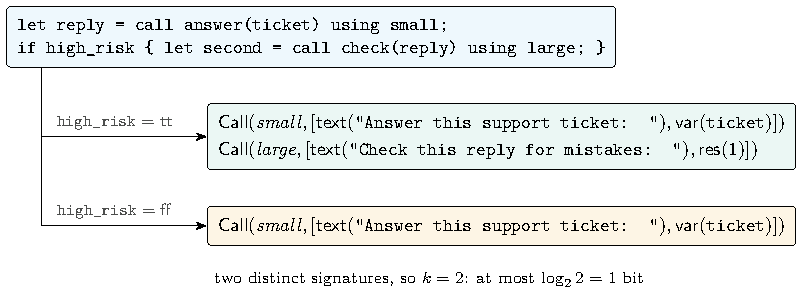
\includegraphics[width=\textwidth]{fig-resolution.pdf}
\caption{Resolution of the running example. The guard \code{high\_risk} reads secret
content, so the analysis inlines each arm the secret can select. The two resulting
signatures differ in their second call, so $k = 2$: the workflow is rejected with
\code{E236}, or accepted with a one-bit budget (\code{leaks 1}). The response of the first
call appears as $\pres(1)$, not as text, because its content is the same in both
executions whatever it is. (Diagram drawn in TikZ with the help of Claude, Anthropic.)}
\label{fig:resolution}
\end{figure}

\begin{example}\label{ex:triage-signature}
\Cref{fig:resolution} resolves \cref{fig:triage}. The first call contributes
\[
\Call(\mathit{small}, [\ptext(\code{"Answer this support ticket: "}), \pvar(\code{ticket})])
\]
to both resolutions. With $\code{high\_risk} = \mathsf{tt}$ the second call is inlined
with the piece $\pres(1)$ for \code{reply}; with $\mathsf{ff}$ nothing is. The two
signatures differ, so $k = 2$. The compiler's message in \cref{fig:triage} prints
exactly this difference.
\end{example}

\subsection{Noninterference}\label{sec:ni}

\begin{lemma}[Equal signatures, equal histories]\label{lem:equal}
Let $\sigv{v_1}(c_1) = \sigv{v_2}(c_2)$, where $v_i$ is the outcome vector of store
$\sigma_i$, and let $\sigma_1$ and $\sigma_2$ agree on every binding that occurs in a
$\pvar$ piece. Then for every tape and every common history, running $c_1$ from
$\sigma_1$ and $c_2$ from $\sigma_2$ under the global, model or request scheme extends
the history by the same events, and binds equal values at corresponding positions.
\end{lemma}

\begin{proof}[Proof sketch]
By induction on the signature. At a call, equal pieces denote equal text: $\ptext$
pieces directly, $\pvar$ pieces by hypothesis, and $\pres$ pieces by the induction
hypothesis. The same request therefore goes to the same model from the same
history, the scheme computes the same key, the tape supplies the same draw, and
$\Pi$ returns the same response. At a retry, equal bodies produce equal attempt
transcripts, and $V$ reads the same transcript and draw, so both executions stop
after the same attempt. A public branch reads equal values and takes the same arm.
A resolved branch inlines the arm that the store actually takes, since $v_i$ is
$\sigma_i$'s own outcome vector. The full proof is in \ref{app:proofs}.
\end{proof}

\begin{theorem}[Request-trace noninterference]\label{thm:ni}
If $k(c) = 1$, then $c$ is pointwise \code{trace}-noninterfering under the global,
model and request schemes, and hence $O$-noninterfering for every provider in
$\Prov$, every tokenizer, every envelope and every observer $O$ that is a function
of the history.
\end{theorem}

\begin{proof}
Take related stores $\sigma_1 \sim \sigma_2$ with outcome vectors $v_1, v_2$. Both
vectors are feasible, so $\sigv{v_1}(c) = \sigv{v_2}(c)$ when $k(c) = 1$. For the
whole workflow every $\pvar$ piece is a public input or a declassified value, on
which the stores agree. \Cref{lem:equal} with the empty history gives equal histories
on every tape, \cref{lem:coupling} turns this into equal distributions, and every
observer is a function of the history.
\end{proof}

No assumption about tokenizers is used. Equal histories contain equal request
texts, and any tokenizer bills equal texts equally; that is the practical
difference from comparing sizes, which is only as good as a tokenizer assumption
and, by \cref{thm:size-blind}, not even that good. In the terms of probabilistic
relational Hoare logic~\cite{barthe2009formal}, \cref{lem:equal} is a derivation
in which every provider call is related by the identity coupling on its draw. The
sampling rule that justifies such a step requires the two distributions to be equal
up to a bijection, and with the identity bijection they must be identical. Requests
with equal content satisfy this; requests with equal size do not, and read as such
a derivation the size rule applies the rule to two different distributions. More broadly, comparing two resolutions is a specialised form of
self-composition~\cite{Barthe2004SelfComposition,Terauchi2005Safety,Barthe2016ProductPrograms}
in which the product program never has to be built, because the signatures are
compared directly.

\subsection{Quantitative leakage}\label{sec:quantitative}

Rejecting every workflow with $k(c) > 1$ is too strict for workflows that must reveal
a little, such as a service tier that selects a larger model for paying
customers. A workflow may declare a budget \code{leaks} $b$, and it is accepted with
warning \code{W238} if $k(c) \leq 2^b$.

\begin{theorem}[Leakage bound]\label{thm:leakage}
For every provider in $\Prov$, every fresh keying scheme and every observer of the
history, together with the workflow's outputs and effects, the channel from the
secrets to the observer has min-capacity at most $\log_2 k(c)$. The bound holds for
any number of invocations with the same secrets and any public inputs, including
public inputs chosen adaptively from earlier observations.
\end{theorem}

\begin{proof}[Proof sketch]
Partition the secret assignments by the class of their signature; there are at
most $k(c)$ classes. By \cref{lem:equal}, two assignments in one class produce equal
histories on every tape and for every public input, since signatures are symbolic
in the public inputs. Outputs and effects are functions of public data and
responses, because the type system rejects any output or effect under a secret
program counter (\cref{fig:rules}). Each invocation's observation is therefore a
function of the class, the public inputs and the tape, and over adaptively chosen
invocations the whole observation sequence is a function of the class, the tapes
and the adversary's coins. The channel is a cascade whose first stage is a
deterministic map onto at most $k(c)$ classes. The min-entropy leakage of a cascade
is at most that of its first stage~\cite{espinoza2012min}, and for every prior the
min-entropy leakage of a channel with at most $k$ possible outputs is at most
$\log_2 k$~\cite[Theorem 1]{doychev2013cacheaudit}; see also~\cite{kopf2010vulnerability}.
\ref{app:proofs} gives the details.
\end{proof}

The argument follows Köpf and Basin's model of an adaptive attacker as a partition
of the secrets into classes the attacker cannot tell apart~\cite{kopf2007information},
with signature classes in place of observations. Counting observations would
be useless here, since the provider's noise gives every workflow with a call a vast
number of possible observations; that is why the interval bound of
\cref{sec:classical} is vacuous. The coupling removes the noise from the count.

\subsection{Coarser observers, and an unsound optimisation}\label{sec:coarser}

A bill does not record order, and a provider sees only its own requests. The
\emph{provider normal form} of a signature stably sorts, by provider, every maximal
run of calls none of which references another in the run, outside any retry body,
and rewrites $\pres$ references to follow the moved calls. The \emph{bill normal
form} sorts such runs by the full request.

\begin{theorem}[Coarser observers]\label{thm:observers}
If the provider (bill) normal forms of $\sigv{v}(c)$ agree for all feasible $v$, then
$c$ is pointwise \code{provider}- (\code{bill}-) noninterfering under the request
scheme, and hence \code{provider}- (\code{bill}-) noninterfering.
\end{theorem}

Under the request scheme a call's draw is keyed by its request and occurrence, not
by its position, so a stably sorted run sends the same multiset of requests and
each copy of a request receives the same response. Calls inside a retry body are
not reordered: the validator sees an attempt's transcript in order, and it may
depend on the order. An intermediate version of our analysis did reorder there. It
accepted a workflow for which, under the same seed, the runtime made one attempt
for one value of the secret and three for the other. The workflow is now a regression
test.

\subsection{Completeness relative to dead code}\label{sec:completeness}

\begin{theorem}[Relative completeness]\label{thm:completeness}
Suppose $\sigv{v_1}(c) \neq \sigv{v_2}(c)$ for feasible $v_1, v_2$, and every public
guard on the path to the first difference can go either way for some public inputs
and responses. Then some provider in $\Prov$ distinguishes the two secrets. For
$k(c)$ classes, some provider and prior attain the bound of \cref{thm:leakage}.
\end{theorem}

\begin{proof}[Proof sketch]
Choose public inputs that are distinct fresh strings, and a provider whose responses
are fresh strings encoding the request and the draw, with a validator that always
fails. Rendering signatures to histories is then injective, and the histories agree
up to the first difference by \cref{lem:equal}.
\end{proof}

A rejection is therefore justified, except when the difference sits under a public
guard that can never go the relevant way. One consequence concerns two different
public variables of equal declared length. A size-based rule accepts a branch that
sends one in each arm; the content rule rejects it, and \cref{thm:completeness} says
the rejection is required, because the variables can hold different text and some
provider answers them differently.

\section{Token bounds that hold for real tokenizers}\label{sec:bounds}

A worst-case bound on the tokens a workflow is billed for has an output side and an
input side. The output side is easy, because providers enforce a model's output cap
themselves. The input side is where the obvious composition,
$\tok(\text{template}) + \sum \tok(\text{argument})$, fails.

The combinators of our bound are the textbook ones for a structured
language~\cite{Wegbreit1975}: a sum for sequencing, a maximum for a branch,
and multiplication for a bounded loop, as in cost-relation analyses of bytecode and
of workflow models~\cite{Albert2012CostBytecode,ali2023cost}. What is new is the measure. In
a workflow model such as Rpl the cost of a step is declared by the
program~\cite{ali2023cost}; in an LLM workflow the cost of a call is decided by a
tokenizer the program does not control, applied to text the program only partly
knows.

\subsection{What fails}\label{sec:what-fails}

We measured fourteen tokenizers, each pinned to an exact revision: GPT-2, the
\code{r50k\_base}, \code{cl100k\_base} and \code{o200k\_base} encodings of
tiktoken~\cite{tiktoken}, and the tokenizers of Llama~2 and~3, Mistral, Phi-3,
Gemma~2, Qwen2.5, DeepSeek-V3, OLMo~2, T5 and XLM-R loaded through Hugging Face
\code{tokenizers}~\cite{hftokenizers}. The inputs were every Unicode scalar value,
388 texts of the Universal Declaration of Human Rights in 360
languages~\cite{udhr2corpus}, twelve source files and eight JSON files. Four facts
emerged.

\begin{enumerate}[leftmargin=*]
\item \emph{Tokenization is not subadditive.} $\tok(u \cdot v) - \tok(u) - \tok(v)$
  reaches 3 to 6, depending on the tokenizer. Under \code{cl100k\_base},
  \code{" Attribute"} and \code{"profiles"} are one token each, and
  \code{" Attributeprofiles"} is six.
\item \emph{Responses inflate when re-encoded.} Decoding generated tokens to text and
  encoding the text again with the same tokenizer yields up to nine tokens per
  generated token (Qwen2.5), so a model's output cap does not bound the length of
  its response as input to the next call.
\item \emph{Tokens can outnumber bytes.} The bound $\tok(s) \leq \bytes(s)$ fails for six
  of the fourteen tokenizers. SentencePiece tokenizers add a dummy prefix that no
  byte pays for, Qwen2.5 normalises its input to NFC and turns the three-byte
  character U+0FAC into six tokens, and the normalisers of T5 and XLM-R, which
  resemble NFKC, produce up to 194 more tokens than bytes on one string.
\item \emph{The usual estimate is only an estimate.} A compiler can compute
  $\lceil\bytes/4\rceil$, and that estimate is exceeded on 67.0--99.8\% of
  256-character windows of the multilingual texts and on 45.7--95.1\% of windows of
  source code, depending on the tokenizer (\cref{fig:tokenizers}).
\end{enumerate}

\begin{figure}[t]
\centering
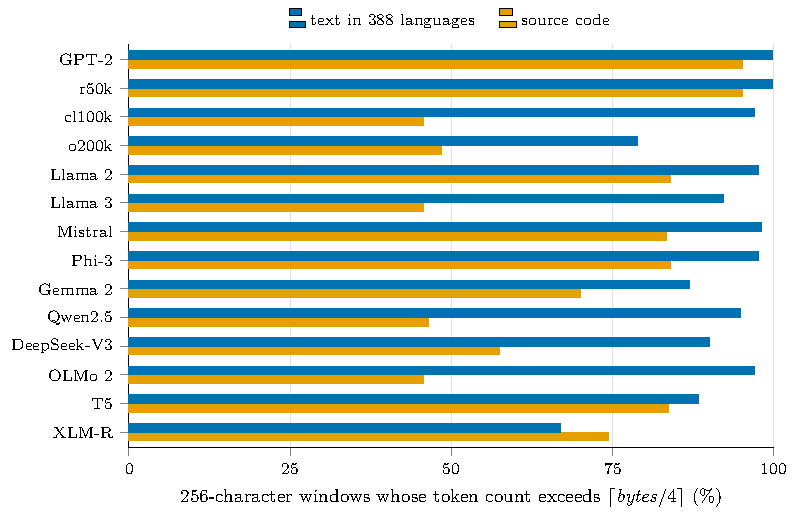
\includegraphics[width=\textwidth]{fig-tokenizers.pdf}
\caption{Share of 256-character windows whose token count exceeds $\lceil\bytes/4\rceil$,
for each of the fourteen tokenizers. The estimate fails on most multilingual text for every
tokenizer, and on almost all source code for the older byte-level encodings (GPT-2,
\code{r50k}) and the SentencePiece tokenizers. The data are those of
\file{bench/results/tokenizers.json}.}
\label{fig:tokenizers}
\end{figure}

These are not new observations about any one tokenizer: that tokenizers charge
languages very unequally is well documented~\cite{petrov2023language}. The point is
their consequence for bounds. A bound assembled from per-part token counts is not a
bound, and neither is one that treats the previous call's output cap as its
response's input cost.

\subsection{Bytes and contracts}\label{sec:contracts}

Bytes add up under concatenation, and they do not depend on the tokenizer. OrchLang
therefore computes each request's length in bytes, as the template's bytes plus the
byte bound of each argument, and converts to tokens once per request, through a
contract for the model's tokenizer.

\begin{definition}[Tokenizer contract]\label{def:contract}
A tokenizer $\tau$ satisfies the \emph{contract} $(\kappa, \sigma)$ if
$\tau(s) \leq \kappa \cdot \bytes(s) + \sigma$ for every string $s$. Its \emph{expansion}
$\lambda_\tau$ is the largest number of bytes that one vocabulary entry decodes to.
\end{definition}

For a byte-level BPE tokenizer, $\kappa = 1$ and $\sigma = 0$ hold structurally, because
every token covers at least one byte. A SentencePiece tokenizer with byte fallback
needs a small $\sigma$ for its dummy prefix and special tokens. Qwen2.5 needs
$\kappa = 3$, because it tokenizes after NFC normalisation, and Unicode's stability
policy guarantees that normalising a string to NFC never makes it more than three
times longer in UTF-8~\cite[Section 9]{uax15}. T5 and XLM-R have no structural
contract; the compiler lets a workflow name them but warns (\code{W267}) and leaves
the guaranteed bound undefined. \Cref{tab:contracts} lists the contracts, which a
script generates from the measurements; it refuses to emit any contract that a
measurement contradicts.

\begin{table}[t]
\centering
\caption{Tokenizer contracts used by the compiler: $\tau(s) \leq \kappa\cdot\bytes(s) + \sigma$,
and $\lambda$ bytes at most per decoded token. The contracts are structural arguments checked
against exhaustive per-code-point measurements; they are not proofs.}
\label{tab:contracts}
\footnotesize
\begin{tabularx}{\textwidth}{@{}>{\raggedright\arraybackslash}X>{\raggedright\arraybackslash}p{4.4cm}ccc@{}}
\toprule
Tokenizers & Family & $\kappa$ & $\sigma$ & $\lambda$ \\
\midrule
GPT-2, \code{r50k}, \code{cl100k}, \code{o200k}, DeepSeek-V3, OLMo~2 & byte-level BPE & 1 & 0 & 128 \\
Llama~3 & byte-level BPE & 1 & 1 & 128 \\
Qwen2.5 & byte-level BPE after NFC & 3 & 0 & 128 \\
Llama~2, Mistral & SentencePiece BPE, byte fallback & 1 & 2 & 27, 25 \\
Phi-3 & SentencePiece BPE, byte fallback & 1 & 1 & 27 \\
Gemma~2 & SentencePiece BPE, byte fallback & 1 & 1 & 48 \\
T5, XLM-R & SentencePiece Unigram, NFKC-like & \multicolumn{2}{c}{none} & 18, 48 \\
\bottomrule
\end{tabularx}
\end{table}

The byte length of a response of $o$ output tokens is at most $\lambda_\tau \cdot o$,
provided decoding a sequence of tokens, with invalid UTF-8 replaced by U+FFFD, never
yields more bytes than decoding its tokens separately. We checked this property
exhaustively on all byte strings of length at most three and on 300,000 random
pairs, but did not prove it. A model may also declare a client-side byte cap
(\code{max\_bytes}), which then replaces the product.

\begin{theorem}[Guaranteed bound]\label{thm:bound}
Assume that each provider reports at most its model's cap, that each tokenizer
satisfies its contract, that each envelope adds at most the declared overhead, that
each input satisfies its declared byte bound, and that each response has at most
$\lambda \cdot \capm$ bytes, or at most the declared byte cap. Then in every execution
the output tokens and the billed input tokens are at most the certificate's
\code{output\_tokens} and \code{input\_tokens\_guaranteed}, and their sum is at most
its guaranteed total.
\end{theorem}

\begin{proof}
By induction on the command, combining bounds by a sum for sequencing, a
componentwise maximum for a branch (for the total, the maximum of the arms'
totals) and multiplication by $n$ for \code{retry} $n$, since a body runs at most
$n$ times. For a call, the output count is at most the cap by assumption, and the
billed input is $\tau_m(q) + \mathit{env} \leq \kappa \cdot \bytes(q) + \sigma +
\mathit{overhead}$. The quantity $\bytes(q)$ is the template's bytes plus the bytes of
the arguments, each bounded by its literal length, by the input's declaration, or by
the response bound of the previous call. Arithmetic saturates, which only rounds
up, and a saturated bound is rejected.
\end{proof}

The proof is mechanised as \code{unary\_bound} and \code{guaranteed\_bound}, with the
assumptions as hypotheses (\cref{sec:mechanisation}). The contracts and $\lambda$ are
measured, not proved: that $\tau(s) \leq \kappa \cdot \bytes(s) + \sigma$ holds for
\emph{every} string rests on the structural argument, which the per-code-point
measurement checks but cannot establish.

\begin{example}\label{ex:triage-bound}
Take the variant of \cref{fig:triage} with a one-bit budget, which the compiler
accepts. Its first request is at most 28 template bytes plus 4,096 bytes of ticket, so it is billed at most $4{,}124 + 9 = 4{,}133$ input tokens under
\code{o200k\_base}. The second request contains the first response, which may decode to
$128 \times 300 = 38{,}400$ bytes, so its guaranteed input is $31 + 38{,}400 + 9 =
38{,}440$ tokens, while the estimate counts that response as 300 tokens. The
certificate records a guaranteed input bound of 42,573 tokens, against an estimate of
1,341.
\end{example}

The price of soundness is $\lambda$. A response of 4,096 tokens may decode to
512\,KiB, and a chain of calls compounds it. On the real workflows the guaranteed
bound is four times the estimate where requests carry only inputs and up to 128 times
the estimate where they carry earlier responses (\cref{sec:eval-real}). A client-side
byte cap on the model is the practical remedy.

\section{Mechanisation}\label{sec:mechanisation}

We mechanised the core of the development in Coq~8.18~\cite{coq818}. The file
\file{proofs/OrchLang.v} has about 1,100 lines, uses no axioms, and builds in a few
seconds with \code{make proofs}, which also runs \code{Print Assumptions} on each
main theorem; every one is reported closed under the global context.
\Cref{tab:coq} maps the results of this paper to their Coq names.

\begin{table}[t]
\centering
\caption{Results of this paper and their mechanisation. ``Pen and paper'' results have full
proofs in \ref{app:proofs}.}
\label{tab:coq}
\footnotesize
\begin{tabular}{@{}lll@{}}
\toprule
Result & Coq & Status \\
\midrule
\Cref{lem:coupling} (coupling validity) & & pen and paper \\
\Cref{thm:size-blind} (size blindness) & \code{size\_blind} & mechanised \\
\Cref{lem:equal} (equal signatures) & \code{equiv\_sound} & mechanised \\
Resolution by a store's outcomes & \code{resolve\_exact} & mechanised \\
\Cref{thm:ni} (noninterference) & \code{request\_trace\_noninterference}, & mechanised \\
 & \code{observers\_agree} & \\
\Cref{thm:leakage} (leakage bound) & & pen and paper \\
\Cref{thm:observers} (coarser observers) & & pen and paper \\
\Cref{thm:completeness} (completeness) & & pen and paper \\
\Cref{thm:bound} (guaranteed bound) & \code{unary\_bound}, & mechanised \\
 & \code{guaranteed\_bound} & \\
\bottomrule
\end{tabular}
\end{table}

\paragraph{What is modelled} The development covers the core calculus of
\cref{sec:providers}: calls, public and secret branches, and retry. The provider
\code{Pi}, the validator \code{V}, the keying scheme, the tape and the guard
predicates are section variables, so every theorem holds for all of them.
\Cref{fig:coq} shows the mechanised statement of \cref{thm:ni}. The relation
\code{bequiv} is a request-equivalence judgment: a derivation of it for the two
resolved programs is the Coq counterpart of equal signatures, and
\code{equiv\_sound} is \cref{lem:equal}. Strings are Coq strings, so length is a length
in bytes. The store is flat, and block scoping appears as freshness side conditions
of the judgment, which the implementation meets by giving every declaration its own
identity. \Cref{thm:bound} is stated with the tokenizer contract, the decoding bound
$\lambda$ and the provider's cap as hypotheses (\code{Pi\_cap}, \code{Pi\_bytes},
\code{bin\_contract}), so the theorem is exactly as strong as those measured facts.

\begin{figure}[t]
\begin{lstlisting}[language={},numbers=none,xleftmargin=0pt,basicstyle=\ttfamily\scriptsize,
  morekeywords={Theorem,forall,Proof,Qed}]
Theorem request_trace_noninterference :
  forall (b : block) (pubs : list var) (s1 s2 : store) (v1 v2 : guard -> bool) G',
    (forall x, In x pubs -> s1 x = s2 x) ->   (* related stores           *)
    agrees v1 s1 -> agrees v2 s2 ->           (* each vector is its store's *)
    no_secret_assign_block b ->
    bequiv (diag pubs) (resolve_block v1 b) (resolve_block v2 b) G' ->
    forall h, snd (exec_block b s1 h) = snd (exec_block b s2 h).
\end{lstlisting}
\caption{The mechanised form of \cref{thm:ni}. If the two resolutions of \code{b} are
request-equivalent, executions from related stores extend any history by the same events,
for every provider \code{Pi}, validator \code{V}, keying scheme and tape, all of which are
section variables. The corollary \code{observers\_agree} applies any function of the history.}
\label{fig:coq}
\end{figure}

\paragraph{What is not mechanised} \Cref{lem:coupling} is not mechanised, so the Coq
theorems are pointwise, per tape. \Cref{thm:leakage,thm:observers,thm:completeness}
are pen and paper. That equal signatures, as the implementation computes them, give a
derivation of \code{bequiv} is argued in the text rather than proved, and the C++
implementation is not verified against the model; it is connected to it only by the
tests and the evaluation of \cref{sec:evaluation}. A route to closing that gap is
the one Miculan took for a flow logic of KLAIM: mechanise the analysis itself and
extract a checker that decides exactly the judgment the theorems are
about~\cite{Miculan2027Klaim}.

\paragraph{A gap found} Mechanising \cref{thm:size-blind} exposed the flaw in our
first definition of fresh twins that \cref{sec:theorem} describes. The pen-and-paper
proof had assumed, without saying so, that a string absent from every constant is
absent from every concatenation of constants. The Coq proof needs the stronger
property, a character that occurs in no constant, in the lemma
\code{marked\_request}, and stating that lemma is what revealed the gap.

\section{Implementation}\label{sec:implementation}

The compiler \code{orchc} is about 7,900 lines of C++17 with no dependencies
(\cref{fig:pipeline}). A recursive-descent parser with error recovery feeds a
semantic analysis that assigns binding identities and computes both labels of every
value. The cost analysis derives the output bound, the estimated input and the
guaranteed input of \cref{sec:bounds}; the relational analysis computes signatures,
resolves secret branches and checks the leakage budget. The two withdrawn rules of
\cref{sec:failed} remain in the code base as selectable baselines
(\code{--relational-rule bounds|sizes}), so that the evaluation can run all three on
the same workflows. The certificate emitter writes the JSON certificate of
\cref{sec:language}, which records the analysis version, the relational rule used and
the SHA-256 digest of the source. \code{make check} builds with
\code{-Wall -Wextra -pedantic} and runs 137 tests, among them every counterexample
from both audits.

\begin{figure}[t]
\centering
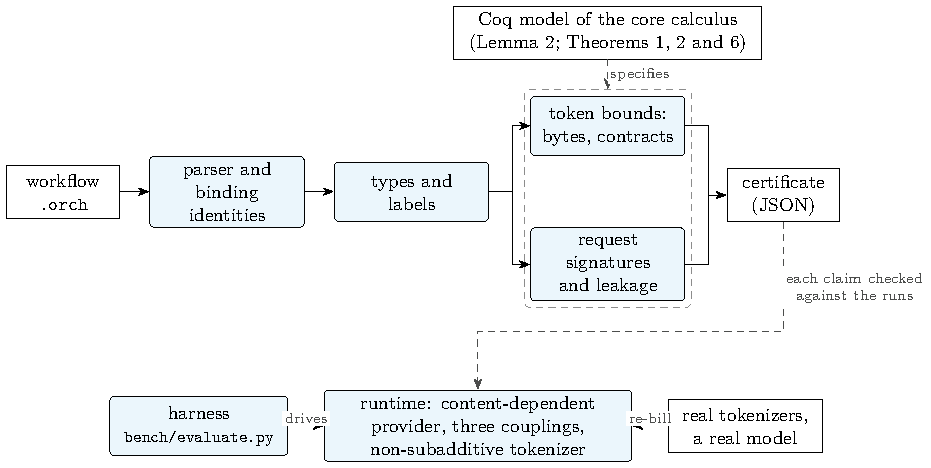
\includegraphics[width=\textwidth]{fig-pipeline.pdf}
\caption{Architecture. The compiler checks a workflow in three stages and emits a
certificate; the harness then runs every workflow under the mock runtime and checks each
claim of the certificate against the runs, re-billing requests with real tokenizers. The Coq
model specifies the two analyses for the core calculus but is not connected to the C++ code.
(Diagram drawn in TikZ with the help of Claude, Anthropic.)}
\label{fig:pipeline}
\end{figure}

\paragraph{A runtime built to falsify the analyses} The first version of the
runtime shared the blind spot of the rule it was meant to test. It drew every output
length uniformly at random, whatever the request said, and billed input with the
analysis's own estimate. Those are exactly the assumptions under which comparing
sizes is sound, so that runtime could not have revealed the failures of
\cref{sec:failed}. The current runtime has a content-dependent provider mode, in
which each draw is mixed with a hash of the request, so any change to a request
changes the answer. Its mock tokenizer uses greedy longest match over a small
vocabulary with overlapping entries, so it is not subadditive, as real tokenizers are
not. It implements the three keying schemes of \cref{sec:couplings}, and it bills
per model name as a provider's invoice would. With \code{run --json} it emits the
full transcript, which is what the harness compares.

\paragraph{The harness} The script \file{bench/evaluate.py} checks every relational
verdict under every combination of provider mode, keying scheme and accounting mode,
re-bills recorded requests with real tokenizers, and exits with a nonzero status on
any violation of a certificate. It too was rewritten: an earlier version skipped
failing cases, counted any nonzero exit of the compiler as a detected leak, and
returned success despite recorded violations. A harness that cannot fail cannot
support a claim, so we tested checks by breaking the property they check; for
instance, the check that a ported prompt occurs in its source was run against a port
into which we had inserted an invented sentence, and it failed as it should.

\paragraph{How the artifact was produced} The compiler, the harness and the Coq
development were written with the help of an AI coding assistant (Claude,
Anthropic), working under the author's direction. We report this here because it
concerns the method: none of the results depends on trusting that process, since
each is reproduced by the artifact's own checks (\code{make check}, \code{make proofs}
and \code{python bench/evaluate.py}), and \cref{sec:evaluation} reports what those
checks print.

\section{Evaluation}\label{sec:evaluation}

The evaluation asks five questions.

\begin{description}[leftmargin=2.6em, style=nextline, itemsep=1pt]
\item[RQ1] Is a certified bound ever exceeded?
\item[RQ2] Does the content rule accept only workflows whose observers cannot tell
  secrets apart, and are its rejections real? How do the two withdrawn rules and the
  classical quantitative bound fare on the same workflows?
\item[RQ3] Are the leakage bounds respected, and how tight are they?
\item[RQ4] What do real tokenizers and a real model say about the assumptions?
\item[RQ5] What happens on real workflows?
\end{description}

\subsection{Setup}\label{sec:eval-setup}

Every number in this section is printed by \code{python bench/evaluate.py}, which exits
with a nonzero status if any assertion fails; \cref{tab:experiments} lists its
experiments. We ran it on a Linux machine with four cores of an Intel Xeon processor
at 2.80\,GHz and 15\,GB of memory, with \code{orchc} built by GCC 13.3, Python 3.11,
tiktoken 0.14.0, Hugging Face \code{tokenizers} 0.20.3 and \code{transformers}
4.46.3~\cite{wolf2020transformers}, and Coq 8.18.0. Every tokenizer, the model and
every source of the real-workflow corpus is pinned to a revision. The plots are drawn by
pgfplots directly from the JSON files that the harness writes, through the script
\file{submission/scp/figures/data.py}, which was written, like the rest of the artifact,
with the help of Claude (Anthropic).

\begin{table}[t]
\centering
\caption{The experiments of \file{bench/evaluate.py}. Each fails the run on any violation.}
\label{tab:experiments}
\small
\begin{tabularx}{\textwidth}{@{}l>{\raggedright\arraybackslash}Xl@{}}
\toprule
& What is checked & RQ \\
\midrule
E0 & counterexamples of both audits are still caught & RQ1, RQ2 \\
E1--E3 & certified bound against 4,600 executions of 23 generated workflows; two simpler bounds for comparison & RQ1 \\
E4 & guaranteed input bound against the content-sensitive tokenizer on byte-bounded variants & RQ1 \\
E5 & three relational rules on 25 workflows, against the observer, under every mode & RQ2 \\
E6 & requests of the size rule's leaking acceptances re-billed with real tokenizers & RQ2 \\
E7 & leakage bounds: certified classes against distinct observations; the interval bound & RQ3 \\
E8 & flow policy on 26 paired secure/insecure workflows & RQ1 \\
E9 & facts about fourteen real tokenizers (\cref{sec:what-fails}) & RQ4 \\
E10 & a real model: output length against request content & RQ4 \\
E11 & 30 real workflows: labels, bounds, re-billing, AgentDojo cross-check & RQ5 \\
\bottomrule
\end{tabularx}
\end{table}

\subsection{RQ1: certified bounds}\label{sec:eval-bounds}

On 23 generated workflows (chains, branches, retries, nesting and wide inputs), 4,600
executions under the estimate model never exceeded the certified total, the output
component or the estimated input component, each checked separately (E1). A flat
per-call sum, which ignores that a retry multiplies its body, was exceeded on 14.9\%
of executions, and a rule that follows control flow but charges a retry body once on
15.4\% (E2). The median slack of the certified bound over the largest observed cost was
1.17, with a range from 1.03 to 1.67 (E3).

The estimate model is the compiler's own, so E4 tests the guaranteed input bound
against something the compiler does not model. On byte-bounded variants of the same
23 workflows, under the content-sensitive tokenizer and both provider modes, the
guaranteed input bound was never exceeded in 4,600 executions, while the estimate was
exceeded in 43.9\% of them. The median slack of the guaranteed bound was 1.85. The
counterexamples of the external audit to the first version of the bound still hold
(E0), and on the 26 workflows of the flow suite every insecure variant was rejected
for a flow reason and every secure variant accepted (E8). The secure variants differ
from the insecure ones by an endorsement or a declassification, which the compiler
records rather than verifies, so E8 measures conformance to the declared policy, not
robustness against adversarial text.

\subsection{RQ2: the content rule and the withdrawn rules}\label{sec:eval-rules}

The relational suite has 25 workflows: 11 whose observers cannot tell the secret
apart, and 14 that leak, among them the audit counterexamples. For each workflow
the harness enumerates every value of the secret under 10 seeds, both provider modes,
the three keying schemes and both accounting modes, and compares what the
workflow's declared observer sees (E5). \Cref{fig:relational} shows the verdicts.
The content rule accepts exactly the 11 leak-free workflows. Across them, 21,080 paired
comparisons showed no difference, and every one of the 14 rejected workflows has a
concrete witness: a seed and a mode under which two values of the secret produce
different observations.

\begin{figure}[t]
\centering
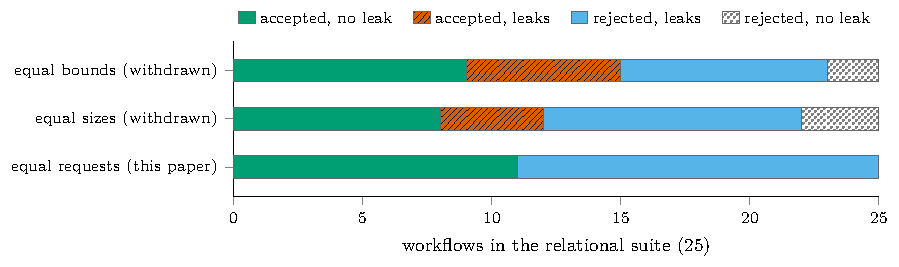
\includegraphics[width=\textwidth]{fig-relational.pdf}
\caption{Verdicts of the three relational rules on the 25 workflows of the relational suite,
against what the runtime shows. The two withdrawn rules accept leaking workflows (hatched);
the content rule accepts only the 11 workflows whose observer never distinguishes the secrets,
and each of its 14 rejections has a witness.}
\label{fig:relational}
\end{figure}

The bounds rule accepts 15 workflows, six of which leak, and the size rule accepts
12, four of which leak. The configuration of the harness before this work (uniform
provider, global keying and estimated billing) detects only one of the size rule's
four leaking acceptances, the one in which the model differs between the arms: the
blind spot of \cref{sec:implementation}, measured. With the provider's answers held
fixed, three of the four leaking acceptances already bill differently under real
tokenizers (E6). The fourth, a redeclared prompt, sends requests of equal token
counts under all three tokenizers, so its leak shows only through a provider that
reads content. Finally, the interval-counting bound of Ngo et al.\ gives between 6.0
and 9.4 bits on the 11 workflows that the content rule proves leak-free, where the
certified bound is zero (E7).

\subsection{RQ3: leakage bounds}\label{sec:eval-leakage}

The leakage suite has eight workflows whose branches test one or two secrets, as
flags or as length intervals, with budgets of 0 to 2 bits (\cref{tab:leakage}). For every workflow, the
number of distinct observations produced by any seed and mode never exceeded the
certified number of classes, and it reached that number in every case: the bound is
attained, as \cref{thm:completeness} predicts. The three workflows whose classes
exceed their budget are rejected.

\begin{table}[t]
\centering
\caption{Leakage suite (E7): declared budget, certified classes and bits, and the largest
number of distinct observations of the trace produced by any seed and mode. The last column
is Ngo et al.'s interval bound, in bits, for the same workflow.}
\label{tab:leakage}
\footnotesize
\begin{tabular}{@{}lrrrrrr@{}}
\toprule
Workflow & Verdict & Budget & Classes & Bits & Observed & Interval \\
\midrule
BalancedNoLeak & accept & 0 & 1 & 0 & 1 & 7.67 \\
ChainedEscalation & accept & 1 & 2 & 1 & 2 & 9.89 \\
FourIntervals & accept & 2 & 4 & 2 & 4 & 9.13 \\
OneBitTier & accept & 1 & 2 & 1 & 2 & 8.42 \\
TwoFlagsThreeClasses & accept & 1.6 & 3 & 1.585 & 3 & 7.75 \\
FourIntervalsOneBit & reject & 1 & 4 & 2 & 4 & -- \\
OneBitNoBudget & reject & 0 & 2 & 1 & 2 & -- \\
TwoFlagsBudgetTooSmall & reject & 1.5 & 3 & 1.585 & 3 & -- \\
\bottomrule
\end{tabular}
\end{table}

\subsection{RQ4: real tokenizers and a real model}\label{sec:eval-models}

The tokenizer facts of \cref{sec:what-fails} are E9, and the harness re-checks the
headline examples live. For the provider assumption, \file{bench/provider/measure.py}
runs SmolLM2-135M-Instruct~\cite{allal2025smollm2,smollm2instruct135m} locally, at a
pinned revision, on fifteen pairs of chat requests padded to exactly equal token
counts under the model's own tokenizer and chat template (E10). Under a shared
sampling seed, all fifteen pairs produced outputs of different lengths, with a mean
absolute difference of 34.1 tokens, while identical requests with the same seed gave
identical outputs in all six trials. Output length is a function of content, not
size, which is exactly the freedom \cref{thm:size-blind} gives the provider. The model
is small, and E10 shows that a real model behaves this way, not how often or by how
much a hosted one does.

\subsection{RQ5: real workflows}\label{sec:eval-real}

\paragraph{Corpus and protocol} The candidates are every workflow defined by the
agent-pattern notebooks of the Anthropic cookbook (7)~\cite{claudecookbooks}, every
LangGraph tutorial notebook (25)~\cite{langgraphrepo}, and the first five user tasks of
each suite of AgentDojo~v1 (20)~\cite{debenedetti2024agentdojo,agentdojorepo}, each
source pinned to a commit. The protocol, the candidate list, the split and every label
were committed before any port was written. Labels are properties of the source,
derived by fixed rules: content from outside the workflow's trust boundary is
untrusted, and for AgentDojo a tool response is untrusted exactly when AgentDojo's own
canary injections reach it; a secret is data that the source itself treats as
confidential. The expected diagnostics follow from the labels: \code{E233} when
untrusted content reaches an effect's argument, \code{E235} when it decides whether an
effect runs, and \code{W237} for a branch guarded by untrusted data whose arms have
different costs. A candidate belongs to the development split if the first
hexadecimal digit of the SHA-256 of its identifier is between 0 and 4 (15 candidates),
and to the held-out split otherwise (37). We wrote the development ports first, then
froze the compiler and checked the 22 held-out ports once against it. The harness fails
if the compiler changed after the freeze without a declared reason, if a candidate is
in the wrong split, if a labelled diagnostic is missing, or if a stretch of prompt text
of at least 20 characters does not occur in the pinned source.

\paragraph{Expressiveness} We ported 30 candidates and excluded 22, each with a
category fixed in advance: the model chooses which node, tool or agent runs next (9);
interactive input, concurrency or timing (4); duplicates that differ only in the model
backend (4); cyclic graphs with more than one back edge (2); reads whose number the
model chooses (1); iteration over a data-dependent count (1); multimodal input (1).
All 20 AgentDojo tasks were ported, as their ground-truth plans executed as fixed
workflows, which is the plan-then-execute pattern~\cite{beurerkellner2025design}
rather than AgentDojo's tool-calling agent. Four of the seven cookbook workflows and
six of the 25 LangGraph tutorials were ported (\cref{tab:corpus}). Seven ports needed
an adaptation that the language forces, such as passing a whole response where the
source extracts one field, or dropping an early exit decided by a response; each is
recorded with whether the certified bound still bounds the source. Five
self-correction loops had to be unrolled, because a \code{retry} body cannot see its
earlier attempts. Porting also forced one change to the language during the
development split: templates could not contain literal braces, so no JSON schema could
be written verbatim, and \code{\{\{} and \code{\}\}} were added as escapes.

\begin{table}[t]
\centering
\caption{The real-workflow corpus by source (E11). ``Held-out'' counts ported
workflows in the held-out split, ``Errors'' ports labelled with an error, and ``Guarantee''
ports whose guaranteed input bound is defined.}
\label{tab:corpus}
\footnotesize\setlength{\tabcolsep}{4pt}
\begin{tabular}{@{}lrrrrrr@{}}
\toprule
Source & Candidates & Ported & Held-out & Errors & Endorsements & Guarantee \\
\midrule
Anthropic cookbook & 7 & 4 & 2 & 0 & 0 & 0 \\
LangGraph tutorials & 25 & 6 & 4 & 2 & 12 & 4 \\
AgentDojo v1 & 20 & 20 & 16 & 13 & 16 & 20 \\
\midrule
Total & 52 & 30 & 22 & 15 & 28 & 24 \\
\bottomrule
\end{tabular}
\end{table}

\paragraph{Agreement with the labels} Fifteen ports are labelled with an error and
fifteen without. Every labelled error was reported, every port labelled clean was
accepted, and the one warning expected on an accepted port (\code{W237} on a routing
workflow of the cookbook) was reported. Two held-out ports received an \code{E233}
beyond their labelled \code{E235}. In both, a value computed only from trusted data,
inside an arm whose guard is untrusted, inherits the guard's integrity: the program
counter imprecision that \cref{sec:labels} removes for confidentiality but keeps for
integrity. These are false positives against the label rule. We changed the harness
after the freeze so that it reports extra diagnostics as imprecision instead of failing
on them; the protocol records this deviation and the two others made after the freeze,
with what prompted each. The 15 rejected ports are accepted after 28 endorsements in
total, one or two per AgentDojo task, four for a corrective retrieval workflow and
eight for a code-generation assistant. Each endorsement marks a place where the source
lets untrusted content decide an effect.

\paragraph{The AgentDojo cross-check} AgentDojo publishes the runs of its attacks. On the
20 ported tasks, its \code{important\_instructions} attack succeeded against
\code{gpt-4o-2024-05-13} 88 times. Every one of the 88 made a tool call that the task's
plan does not contain, or more calls to a planned effect than the plan makes; none
stayed within the plan. The harness fails on a within-plan success against a task the
checker accepts, and there was none. It is therefore the fixed plan, not the checker,
that excludes every recorded attack. The checker contributes something else: in 13 of
the 20 tasks it marks where untrusted content can still steer a planned effect's
arguments or decide whether it runs. In the bill-payment task, for example, the amount
and recipient of the payment come from a file that an attacker can write. The recorded
attacks did not target those places.

\paragraph{Bounds} All 30 accepted variants are certified. The guaranteed input bound is
defined for 24 and undefined for the six that call a model whose tokenizer is not
published, matching the label in all 30 cases. Each port ran 200 times under the
content-dependent provider and the content-sensitive tokenizer, half of the runs with
every text input at its declared byte bound; in the 6,000 runs neither the output
bound nor the guaranteed input bound was exceeded. Re-billing every run's requests with
the port's real tokenizer never exceeded the guaranteed bound either, and the largest
real bill was 0.24 of it. \Cref{fig:real} shows how loose the guarantee is: 4.0 times the
estimate on every AgentDojo port, whose requests carry only inputs, and 19 to 128 times
on the four LangGraph ports with a guarantee, whose later requests carry earlier
responses and pay $\lambda$ bytes per response token. The estimate is not a bound: the
content-sensitive tokenizer exceeded it in 28--100\% of each port's runs, and the real
tokenizers in none of the AgentDojo runs and in 3.5--41\% of the runs of those four
LangGraph ports. Because the runtime writes inputs and responses from a fixed word list
that includes non-English and invented words, these rates describe the mock text, not
a deployment.

\begin{figure}[t]
\centering
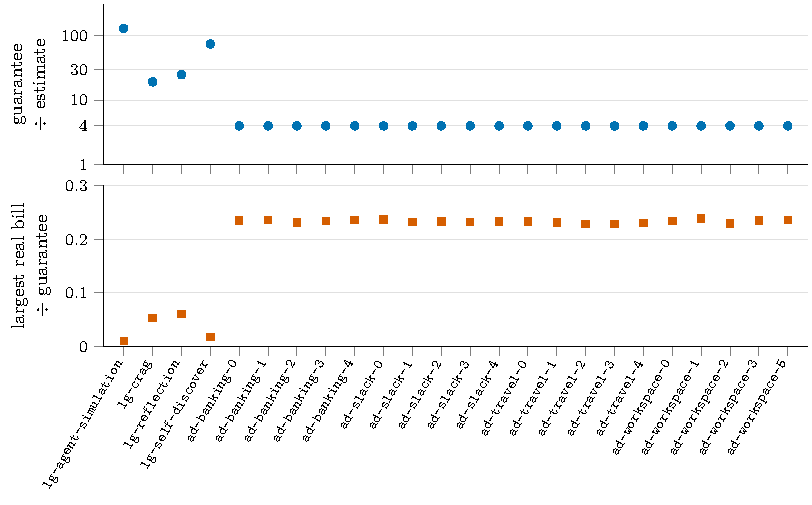
\includegraphics[width=\textwidth]{fig-real.pdf}
\caption{The 24 real ports with a guaranteed input bound. Top: the guaranteed bound
divided by the estimate (log scale); it is 4.0 for every AgentDojo port and 19 to 128 for the
LangGraph ports whose later calls receive earlier responses. Bottom: the largest real-tokenizer
bill in 200 runs divided by the guaranteed bound; no run came within a factor of four of it.}
\label{fig:real}
\end{figure}

\paragraph{The relational analysis} No candidate has a secret, so no port declares one;
\code{E236} and \code{W238} never fired, and every certificate reports a leakage of zero
bits, as it must for a workflow without secrets. On real workflows the relational analysis has, so far, verified
nothing.

\subsection{Analysis cost}\label{sec:eval-cost}

Certifying the 47 synthetic workflows that the harness times takes 0.11\,s in total,
2.4\,ms per workflow, and the 30 real ports, of 17 to 84 lines, take 0.07\,s, the
slowest 3.0\,ms. Both figures include process start-up. The one super-linear step of
the analysis is resolution: the feasible outcome vectors are a product over
independent secrets, each secret contributing a number of vectors linear in its
distinct length thresholds, so their count is exponential in the number of secrets
that guard branches. The implementation enumerates at most 4,096 vectors. Beyond that
it treats every vector as its own class, which keeps \cref{thm:leakage} sound but rejects
a workflow unless its budget covers the logarithm of the vector count. No workflow came
near the limit: the largest number of feasible outcome vectors in any certificate the
harness produces is four.

\subsection{Threats to validity}\label{sec:threats}

\paragraph{Internal validity} The runtime is a mock. Its content-dependent provider is
a hash, which is adversarial in the sense that matters, since any change to a request
changes the answer, but it is not a model; E10 supplies one real model, and a small one.
Re-billing with real tokenizers (E6, E11) applies real tokenizers to the runtime's
requests, whose variable parts are mock text. Relational verdicts are checked by
enumerating declared secret values, which is exhaustive for the suites' small bounds
and would not be for large ones.

\paragraph{Construct validity} The synthetic suites are ours. Their paired design, in
which each unsafe workflow has a safe twin that differs by one edit, stops a checker
from scoring well by rejecting everything, but it does not remove designer bias; the
real-workflow corpus addresses that, but it contains no secrets. The contracts and
$\lambda$ rest on measurement and a structural argument, not on proof, and a tokenizer
revision that changes normalisation could break a contract; for that reason contracts
are tied to revisions and regenerated from measurements.

\paragraph{External validity} The real-workflow corpus draws on three sources and 52
candidates chosen by a fixed rule; it is not a random sample of deployed workflows.
Its labels were derived by rules that we applied ourselves, except that the untrusted
labels of AgentDojo come from AgentDojo's own canary mechanism and the cross-check uses
its recorded runs. The AgentDojo ports are the tasks' ground-truth plans, so neither their
bounds nor the cross-check describe AgentDojo's tool-calling agent. Declared byte bounds
on inputs (8\,KiB where a source gives none) are assumptions that a deployment would
have to enforce. Every assumption the guaranteed bound makes about a provider, its caps
and its envelope overhead, is taken from documentation or framework defaults; no hosted
provider was tested. Finally, the harness's treatment of extra diagnostics was changed
after the held-out results were seen. The change and its cause are recorded, and it
affects only whether the two false positives fail the run, not whether they are
reported.

\section{Related work}\label{sec:related}

\paragraph{Resource-aware noninterference and relational cost} Ngo et al.\ and RelCost
are the closest work and are discussed in \cref{sec:intro-classical,sec:classical}.
Ngo et al.\ extend automatic amortised resource
analysis~\cite{hofmann2003static,hoffmann2012multivariate}, and relational cost analysis
has since been extended to functional-imperative programs~\cite{Qu2019ARel}. Relative to
Ngo et al., our contribution is the theorem that indexing by size cannot be sound for
opaque operations whose cost depends on content. Relative to RelCost, whose refinements
can express the content comparison for a fixed pair of runs, it is the resolution over
feasible secret outcomes, the observers, the leakage bound, and the application to LLM
calls.

\paragraph{Timing channels, constant time and cross-copying} Agat's transformation pads
the arms of a secret branch so that they take equal time~\cite{agat2000transforming}.
The program-counter security model of Molnar et al.\ asks that the sequence of executed
instructions not depend on secrets, and their transformation removes secret-dependent
branches~\cite{molnar2006program}. Constant-time programming forbids secret-dependent
control flow and memory access altogether; it has been checked by
self-composition~\cite{BacelarAlmeida2013SelfComp} and by product
programs~\cite{Almeida2016ConstantTime}. Hermes, a
reversible language for lightweight encryption published in this journal, uses secret and
public types to make operations on secret data independent of it and so to prevent
timing attacks~\cite{Mogensen2022Hermes}. In all of these the observable operation is
fixed by the program: an instruction, a memory access, a step of time. For an LLM call,
the provider fixes the cost from the request content, so ``the same operation'' has to
mean the same request. OrchLang accepts secret branches whose arms send identical
requests and bounds what the remaining differences reveal.

\paragraph{Relational verification} Noninterference is a two-run
property~\cite{goguen1982security}, and self-composition reduces it to a property of one
program~\cite{Barthe2004SelfComposition,Terauchi2005Safety}; product programs connect
such reductions to relational program logics~\cite{Barthe2016ProductPrograms}.
Probabilistic relational Hoare logic~\cite{barthe2009formal} and coupling
proofs~\cite{barthe2017coupling} relate the randomness of two runs. \Cref{lem:equal} is a
derivation of this kind in which every call is related by the identity coupling, and
comparing signatures is a self-composition that never builds the product program.

\paragraph{Quantitative information flow} Min-entropy leakage~\cite{smith2009foundations},
its behaviour under cascading~\cite{espinoza2012min}, bounds by the number of possible
observations~\cite{kopf2010vulnerability,doychev2013cacheaudit}, and the partition model
of adaptive attacks~\cite{kopf2007information} are what \cref{thm:leakage} uses.
CacheAudit bounds cache leakage by counting observations~\cite{doychev2013cacheaudit}; we
count signature classes, because the provider's noise makes counting observations
useless.

\paragraph{Information-flow typing and declassification} OrchLang's flow typing is
conventional: the lattice model of Denning~\cite{denning1976lattice}, the type-based
formulation of Volpano et al.~\cite{volpano1996sound}, and the standard two-point
confidentiality and integrity lattices surveyed by Sabelfeld and
Myers~\cite{sabelfeld2003language}. Its declassification is trusted, justified in writing
and all or nothing: in the dimensions of Sabelfeld and Sands~\cite{SabelfeldSands2009} it
constrains only where in the program a release happens, not what is released or by
whom, and it offers no robustness guarantee~\cite{Myers2006Robust}. In this
journal, Manzino and de Latorre embed a DSL in Haskell whose types enforce delimited
release, so that declassification cannot reveal more than
intended~\cite{manzino2026haskell}, and Ben Said and Cristescu verify noninterference of
web-service compositions and generate secure orchestrators from
them~\cite{BenSaid2020Orchestration}. Both control which data reach which party; neither
addresses what the pattern of an orchestrator's requests reveals.

\paragraph{Static cost analysis and certified bounds} Static cost analysis goes back to
Wegbreit~\cite{Wegbreit1975}; COSTA derives cost relations from bytecode and solves them
into closed-form bounds~\cite{Albert2012CostBytecode}, and Ali, Lamo and Pun apply the
same method to Rpl, a resource-sensitive workflow modelling language, in this
journal~\cite{ali2023cost}. In Rpl the cost of a step is declared by the program, so costs
compose; in an LLM workflow a tokenizer decides it, and token counts do not compose
(\cref{sec:bounds}). Proof-carrying code~\cite{Necula1997PCC} and resource bound
certification~\cite{CraryWeirich2000} attach checkable evidence to a program. OrchLang's
certificate is a report rather than such evidence, and a checker for it is future work.

\paragraph{Languages for LLM programs} LMQL treats prompting as programming, with
constraints on generation~\cite{BeurerKellner2023LMQL}, and DSPy compiles declarative
pipelines of model calls and optimises their prompts~\cite{Khattab2024DSPy}. Both are
more expressive than OrchLang, and neither checks information flow or certifies a token
bound. OrchLang gives up expressiveness, including the agents that make up most of our
exclusions, in exchange for decidable analyses.

\paragraph{Security of LLM agents} Indirect prompt injection~\cite{greshake2023not} is what
the integrity part of OrchLang's typing targets. CaMeL separates a planner from untrusted
data and tracks provenance and capabilities in a custom
interpreter~\cite{debenedetti2026defeating}; FIDES tracks confidentiality and integrity
labels in an agent planner~\cite{costa2025securing}; Beurer-Kellner et al.\ catalogue
design patterns for agents, among them the plan-then-execute pattern that our AgentDojo
ports follow~\cite{beurerkellner2025design}. AgentFlow combines a flow-centric policy
language with a runtime monitor, and explicitly leaves timing, token-length and
resource-usage channels out of scope~\cite{ammanaghattashivakumar2026agentflow}; Ghost in
the Agent tracks information flow through the execution traces of
agents~\cite{cai2026ghost}; Agentproof verifies extracted workflow graphs
statically~\cite{xavier2026agentproof}. None of these bounds resource use or reasons
about what the content of requests reveals. AgentDojo~\cite{debenedetti2024agentdojo}
supplies the tasks and recorded attacks of our evaluation.

\paragraph{Side channels of LLM services} The token lengths of streamed responses leak
response text to a network observer~\cite{weiss2024what}; output token counts leak
information about inputs through timing~\cite{zhang2024time}; the sizes and timing of
encrypted streams reveal prompt topics across 28 models~\cite{mcdonald2025whisper}; and
prompt caches shared across users form a timing channel at seven
providers~\cite{gu2025auditing}. These papers establish the channel for single calls. We
study how a workflow's control flow feeds it.

\paragraph{Budgets and tokenization} Token Budgets catalogues 63 budget-overrun incidents
in LLM agents and enforces spending caps at run time, with affine types that prevent a
budget from being copied or spent twice~\cite{khan2026token}; its over-reservation
figures are measured on a different corpus and are not comparable with our slack.
Tokenizers are known to charge languages very unequally~\cite{petrov2023language}; we
measure what this means for sound bounds.

\section{Limitations and future work}\label{sec:conclusion}

\paragraph{The relational analysis has not met a real secret} None of the 30 real
workflows declares or implies a secret in its source's threat model, so the analysis
that motivates this paper verified nothing on them. The pattern it targets, a branch on
private data that is not itself sent to a model (a customer's tier, a risk flag, the
verdict of a local detector of personal data), is plausible and easy to write, but we
have not shown that deployed workflows contain it. Finding such workflows is the most
important next step.

\paragraph{Declassification is too coarse} Real workflows send private data to a
provider, which in OrchLang requires declassifying it, which makes it public to every
observer. A policy relative to observers, under which the provider may read content
that the network and the bill may not reveal, would let the analysis reason about those
workflows. \Cref{thm:ni,thm:leakage} would then need an equivalence of histories indexed
by observer.

\paragraph{Integrity over-reports} A value computed in an arm guarded by untrusted data
is labelled untrusted even when it is computed only from trusted data. Separating data
and program-counter labels for integrity, as \cref{sec:labels} does for confidentiality,
would remove the two false positives of the held-out split.

\paragraph{Retry cannot carry feedback} Self-correction loops that show the model its
earlier attempts had to be unrolled in five of the thirty ports. A retry whose body can
read an accumulator of declared byte growth would keep the bound finite and express
these loops directly.

\paragraph{Agents are out of scope by design} Thirteen of the 22 exclusions are workflows
whose shape is decided at run time, nine of them because the model chooses what runs
next. OrchLang's fixed shape is what makes its analyses decidable; a type system for
agent loops would need bounds on the model's choices.

\paragraph{The guaranteed bound is loose} On the real workflows it is four times the
estimate where requests carry only inputs and up to 128 times where they carry earlier
responses, unless models declare client-side byte caps.

\paragraph{The certificate is not independently checked, and the implementation is not
verified} A small checker that re-derives the bounds from the certificate and the source,
tested against tampered certificates, would turn the certificate into evidence. The C++
implementation is tested against the Coq model through the runtime, not verified against
it.

\section{Conclusion}\label{sec:conclusion-final}

An analysis that compares LLM requests by anything coarser than their content cannot be
sound against providers that answer content, unless it gives up on every secret branch.
Comparing content gives noninterference that needs no assumption about providers,
tokenizers or observers, and a leakage bound that counts request classes rather than
noisy observations. Token bounds have to be built from the one measure that adds up,
bytes, and converted through tokenizer contracts that measurements can refute. Both
results are mechanised for a core calculus, implemented in a compiler, and tested by a
harness that can fail. On 30 real workflows the bounds held and the flow checks found
the places where untrusted content decides an effect, but the side channel we set out
to close did not appear. Whether it matters in practice depends on whether deployed
workflows branch on private data that they do not send to a model, and that question
remains open.


\appendix
\section{Proofs}\label{app:proofs}

This appendix gives the proofs that \cref{sec:requests} sketches. We use the core
calculus of \cref{sec:providers} and the semantics of \cref{sec:couplings}: given a tape
$\rho$, an execution is deterministic, and $\langle c, \sigma, h\rangle \Downarrow_\rho
\langle \sigma', h' \rangle$ runs $c$ from store $\sigma$ and history $h$. A call
$x \leftarrow \mathsf{call}\ r$ evaluates $r$ in $\sigma$ to a request $q$, computes the
key $k$ of the event from $h$ under the scheme, obtains $(\mathit{resp}, o) = \Pi(m, q,
\rho(k))$, binds $x$ to $\mathit{resp}$ and appends $\mathsf{call}(m, q, \mathit{resp}, o)$.
A retry runs its body, lets $V$ decide from the attempt's transcript and a draw keyed by
it, appends $\mathsf{attempt}(b)$, and stops if $b$ holds or no attempts remain.

\begin{proof}[Proof of \cref{lem:equal}]
By induction on the length of the common signature, and within a node on its nesting.
Throughout, the two executions start from the same history, and we show that they
extend it by the same events and bind equal values at corresponding positions.
\begin{itemize}[leftmargin=*]
\item \emph{Call.} The pieces are equal. A $\ptext$ piece denotes the same text in both
  executions; a $\pvar(b)$ piece denotes $\sigma_1(b) = \sigma_2(b)$ by hypothesis; a
  $\pres(p)$ piece denotes the response bound at position $p$, which is equal in both
  executions by the induction hypothesis. So both evaluate the request to the same text
  $q$ for the same model identity $m$. The histories so far are equal, so the scheme,
  whose keys are functions of the history and the request, computes the same key $k$;
  the tape gives the same draw; and $\Pi(m, q, \rho(k))$ gives the same response and
  count. Both histories are extended by the same event, and both bindings receive the
  same response.
\item \emph{Retry.} The bounds are equal. Each attempt runs a body with equal signatures
  from equal histories, so by the induction hypothesis it produces equal transcripts.
  The validator reads the same transcript and, the histories being equal, the same draw,
  so both executions decide alike and stop after the same attempt.
\item \emph{Public branch.} The guard terms are equal and denote equal values, a $\pvar$
  piece by hypothesis and a $\pres$ piece by induction, so both executions take the same
  arm, whose signatures are equal.
\item \emph{Resolved branch.} $\sigv{v_i}$ inlines the arm that $v_i$ selects, and
  $v_i$ is the outcome vector of $\sigma_i$, so the inlined arm is the one execution $i$
  takes. The inlined nodes are then compared like any others. That a store's own outcome
  vector selects the arm the store takes is \code{resolve\_exact} in the Coq
  development; it needs the side condition that no statement before the branch
  rebinds a secret, which the type system guarantees.\qedhere
\end{itemize}
\end{proof}

\begin{proof}[Proof of \cref{thm:leakage}]
Let $\mathit{cls}(\sigma_S)$ be the class of $\sigv{v(\sigma_S)}(c)$ among the at most $k(c)$
distinct signatures. Fix public inputs $\sigma_P$ and a tape $\rho$. By \cref{lem:equal},
two secret assignments with the same class produce the same history; signatures are
symbolic in the public inputs, so this holds for every $\sigma_P$. Outputs and effects
are functions of public data and responses: the \textsc{Output} and \textsc{Emit} rules
of \cref{fig:rules} reject any output or effect under a secret program counter, and any
secret content reaching them. Hence one invocation's observation is
$G(\mathit{cls}(\sigma_S), \sigma_P, \rho)$ for some function $G$.

Now let an adversary choose the public inputs of each invocation from the observations
of earlier invocations and its own coins $\alpha$, with fresh tapes $\rho_1, \rho_2,
\dots$ By induction on the number of invocations, the whole sequence of observations is
a function of $\mathit{cls}(\sigma_S)$, the tapes and $\alpha$: the $j$-th public input is
a function of the first $j-1$ observations and $\alpha$, and the $j$-th observation is
$G(\mathit{cls}(\sigma_S), \sigma_P^{(j)}, \rho_j)$. The tapes and $\alpha$ are independent
of the secrets. The channel from the secrets to the observations therefore factors as a
cascade whose first stage is the deterministic map $\mathit{cls}$ onto at most $k(c)$
values. The min-entropy leakage of a cascade is at most that of its first
stage~\cite{espinoza2012min}, and for every prior the min-entropy leakage of a channel
with at most $k$ possible outputs is at most $\log_2 k$~\cite[Theorem
1]{doychev2013cacheaudit}. Taking the maximum over priors gives min-capacity at most
$\log_2 k(c)$.
\end{proof}

\begin{proof}[Proof of \cref{thm:observers}]
Consider a maximal run of calls outside any retry body, none of which references
another in the run. Every request in the run is determined by pieces from outside the
run, so both executions send the same multiset of requests in the run (for the bill
normal form) or the same sequence for each provider (for the provider normal form).
Under the request scheme a call's draw is keyed by its model, its request and the
number of earlier calls with the same request, not by its position; a stable sort keeps
equal requests in their order of execution, so the $i$-th copy of a request has the same
occurrence index in both executions and receives the same response. Totals per model
are independent of order, and each provider's own sequence is preserved by the stable
sort. The $\pres$ references are rewritten to follow the moved calls, so later pieces
denote the same responses. Control nodes are compared exactly and sit between runs, so
the induction of \cref{lem:equal} continues past them. Calls inside a retry body are not
moved, because the validator reads the attempt's transcript in order.
\end{proof}

\begin{proof}[Proof of \cref{thm:completeness}]
Choose public inputs that are pairwise distinct strings over a character that occurs in
no constant of the program, and a provider whose responses are fresh strings that encode
the model, the request and the draw, with a validator that always rejects, so every
retry runs to its bound. Under this provider the rendering of a signature as a history
is injective: distinct sequences of pieces give distinct request texts, because the
public inputs and responses are distinct and fresh; distinct retry bounds give distinct
numbers of attempts; and a call present in one signature and absent in the other changes
the length of the history. The hypothesis on public guards provides inputs and responses
that drive both executions to the first difference, before which their histories agree by
\cref{lem:equal}; at the difference the histories differ, so the trace distinguishes the
two secrets. For $k(c)$ classes, the same provider makes the trace an injective function
of the class, a deterministic channel with $k(c)$ distinct outputs, whose min-entropy
leakage under the uniform prior on the classes is $\log_2
k(c)$~\cite[Theorem 1]{smith2009foundations}.
\end{proof}

\begin{proof}[Proof of \cref{prop:pc}]
Under the program-counter rule of Volpano et al.~\cite{volpano1996sound}, an event
observable at the public level may not occur under a secret program counter, and every
call inside a secret-guarded branch occurs under one; so every such branch is rejected.
If calls are unobservable, the rule places no constraint on them, and \cref{fig:triage},
whose only secret-dependent behaviour is a call, is accepted.
\end{proof}

\section{The real-workflow corpus}\label{app:corpus}

\Cref{tab:ports} lists the 30 ports. The adaptations are those of the protocol: A1, a
whole response is passed where the source extracts a field; A2, a multi-way choice
becomes a cascade of yes/no calls; A3, an early exit decided by a response is dropped;
A4, a list that the model filters is passed unfiltered; A6, a stand-in replaces a value
computed inside a branch as the single output. Each adaptation is recorded in the
corpus manifest with whether the certified bound still bounds the source. The 22
excluded candidates, each with its category and reason, are listed in the exclusion log
of the artifact (\file{bench/real/EXCLUSIONS.md}).

\begin{table}[p]
\centering
\caption{The 30 ported workflows (E11). Codes are those reported on the port without
annotations; endorsements are those of the accepted variant. The output bound and the
guaranteed input bound are in tokens; ``--'' means that a model's tokenizer is unpublished.
The last column gives AgentDojo's recorded successful attacks within the task's plan, out of
all successful attacks. Prefixes: \code{ac} Anthropic cookbook, \code{lg} LangGraph,
\code{ad} AgentDojo.}
\label{tab:ports}
\scriptsize\setlength{\tabcolsep}{3pt}
\begin{tabular}{@{}llllrlrrl@{}}
\toprule
Port & Split & Verdict & Codes & End. & Adapt. & Output & Input (guar.) & Attacks \\
\midrule
% Generated by figures/data.py from bench/results/real.json. Do not edit.
\code{ac-chain} & dev & accept & -- & 0 & -- & 16,384 & -- & -- \\
\code{ac-parallel} & dev & accept & -- & 0 & A6 & 16,384 & -- & -- \\
\code{ac-route} & held-out & accept & W237 & 0 & A1 A2 & 16,384 & -- & -- \\
\code{ac-evaluator-optimizer} & held-out & accept & -- & 0 & A1 A3 & 24,576 & -- & -- \\
\code{lg-agent-simulation} & held-out & accept & -- & 0 & A3 & 32,768 & 14,681,956 & -- \\
\code{lg-code-assistant} & dev & reject & E233 E235 & 8 & A1 A6 & 12,288 & -- & -- \\
\code{lg-extraction-retries} & held-out & accept & -- & 0 & A1 A3 & 12,288 & -- & -- \\
\code{lg-crag} & held-out & reject & E233 E235 & 4 & A4 & 73,728 & 642,244 & -- \\
\code{lg-reflection} & dev & accept & -- & 0 & -- & 229,376 & 17,262,535 & -- \\
\code{lg-self-discover} & held-out & accept & -- & 0 & -- & 16,384 & 1,611,298 & -- \\
\code{ad-banking-0} & held-out & reject & E233 & 1 & -- & 8,192 & 17,474 & 0/7 \\
\code{ad-banking-1} & held-out & accept & -- & 0 & -- & 4,096 & 8,716 & 0/7 \\
\code{ad-banking-2} & held-out & reject & E233 & 1 & -- & 8,192 & 33,908 & 0/6 \\
\code{ad-banking-3} & held-out & reject & E233 & 1 & -- & 8,192 & 17,802 & 0/7 \\
\code{ad-banking-4} & held-out & reject & E233 & 1 & -- & 8,192 & 17,478 & 0/7 \\
\code{ad-slack-0} & held-out & accept & -- & 0 & -- & 4,096 & 8,726 & 0/5 \\
\code{ad-slack-1} & dev & reject & E233 & 1 & -- & 12,288 & 42,665 & 0/5 \\
\code{ad-slack-2} & held-out & reject & E233 & 1 & -- & 8,192 & 17,518 & 0/5 \\
\code{ad-slack-3} & held-out & reject & E233 & 1 & -- & 8,192 & 17,516 & 0/5 \\
\code{ad-slack-4} & held-out & reject & E233 & 1 & -- & 12,288 & 42,977 & 0/5 \\
\code{ad-travel-0} & held-out & reject & E235 & 1 & -- & 8,192 & 17,926 & 0/3 \\
\code{ad-travel-1} & held-out & reject & E233 E235 & 1 & -- & 12,288 & 51,861 & 0/2 \\
\code{ad-travel-2} & dev & reject & E233 & 2 & -- & 24,576 & 111,748 & 0/1 \\
\code{ad-travel-3} & dev & reject & E233 & 2 & -- & 16,384 & 85,584 & 0/2 \\
\code{ad-travel-4} & held-out & reject & E233 & 2 & -- & 20,480 & 94,919 & 0/0 \\
\code{ad-workspace-0} & held-out & accept & -- & 0 & -- & 4,096 & 8,800 & 0/6 \\
\code{ad-workspace-1} & held-out & accept & -- & 0 & -- & 4,096 & 8,793 & 0/4 \\
\code{ad-workspace-2} & held-out & accept & -- & 0 & -- & 4,096 & 16,943 & 0/3 \\
\code{ad-workspace-3} & dev & accept & -- & 0 & -- & 4,096 & 8,746 & 0/3 \\
\code{ad-workspace-5} & held-out & accept & -- & 0 & -- & 4,096 & 8,817 & 0/5 \\
\bottomrule

\end{tabular}
\end{table}


%% End matter, in the order Elsevier's guide gives: CRediT, competing interests,
%% data availability, acknowledgements (with funding), generative-AI declaration.
%% TODO(author): confirm the CRediT roles and the funding sentence before submitting.

\section*{CRediT authorship contribution statement}

\textbf{Nambi Rajan M:} Conceptualization, Methodology, Software, Validation, Formal
analysis, Investigation, Data curation, Writing -- original draft, Writing -- review \&
editing, Visualization.

\section*{Declaration of competing interest}

The author declares that they have no known competing financial interests or personal
relationships that could have appeared to influence the work reported in this paper.

\section*{Data availability}

The compiler, the Coq development, the benchmark suites, the real-workflow corpus with
its protocol, exclusion log and labels, and the evaluation harness are openly available at
\url{https://github.com/guyoverclocked/orchlang-compiler-design-project}. The commands
\code{make check}, \code{make proofs} and \code{python bench/evaluate.py} reproduce every
number reported in this paper, and \file{submission/scp/figures/data.py} regenerates the
data behind every plot.
%% TODO(author): archive a tagged release on Zenodo and add its DOI here; add a licence.

\section*{Acknowledgements}

This research did not receive any specific grant from funding agencies in the public,
commercial, or not-for-profit sectors.

\section*{Declaration of generative AI and AI-assisted technologies in the manuscript preparation process}

During the preparation of this work the author used Claude (Anthropic) in order to
develop parts of the compiler, the evaluation harness and the Coq proofs (as described in
\cref{sec:implementation}), to draw the explanatory diagrams, and to draft and edit the
text and check the references against publisher records. After using this tool, the
author reviewed and edited the content as needed and takes full responsibility for the
content of the published article.


\bibliographystyle{elsarticle-num}
\bibliography{references}

\end{document}
